\documentclass[12pt]{amsart}
\usepackage{amsmath,amssymb,amstext,amsgen,amsbsy,amsopn,amsfonts,bbm,graphicx,amsthm,cleveref,mathrsfs,mathtools}

%\usepackage{parskip}
\usepackage[left=3cm, right=3cm, top=3.5cm, bottom=3cm,footskip=1cm,headsep=1.5cm]{geometry}
%example of geometry package \geometry{verbose,tmargin=3cm,bmargin=3.5cm,lmargin=3.5cm,rmargin=3.5cm,headheight=3cm,headsep=4cm,footskip=2cm}
\usepackage[all]{xy}
\usepackage[OT2,T1]{fontenc}
%\usepackage[latin9]{inputenc}
%\usepackage{titletoc}
\usepackage{float}
%\usepackage{relsize}
\usepackage[alphabetic]{amsrefs}
%\usepackage{hyperref}
%\definecolor{darkred}{rgb}{0.5,0,0}
%\definecolor{darkgreen}{rgb}{0,0.5,0}
%\definecolor{darkblue}{rgb}{0,0,0.7}
%\hypersetup{linkcolor=darkblue,filecolor=darkgreen,urlcolor=darkred,citecolor=darkblue}
\usepackage{tikz}

\renewcommand{\baselinestretch}{1}

\crefname{equation}{}{}
\numberwithin{equation}{section}


\newtheorem{theorem}[equation]{Theorem}
\newtheorem{lemma}[equation]{Lemma}
\newtheorem{cor}[equation]{Corollary}
\Crefname{cor}{Corollary}{Corollaries}
\Crefname{example}{Example}{Examples}
\newtheorem{conjecture}{Conjecture}
\newtheorem{proposition}[equation]{Proposition}



\theoremstyle{remark}
\newtheorem{remark}[equation]{Remark}
\theoremstyle{definition}
\newtheorem{example}[equation]{Example}
\theoremstyle{definition}
\newtheorem{construction}[equation]{Construction}
\theoremstyle{definition}
\newtheorem{defi}[equation]{Definition}
\theoremstyle{definition}
\newtheorem{notation}[equation]{Notation}
\theoremstyle{definition}
\newtheorem{convention}[equation]{Convention}
\theoremstyle{definition}
\newtheorem{assumption}[equation]{Assumption}
\newtheorem{exercise}[equation]{Exercise}


\DeclareSymbolFont{cyrletters}{OT2}{wncyr}{m}{n}
\DeclareMathSymbol{\Sha}{\mathalpha}{cyrletters}{"58}
\def\K{\ensuremath K}
\def\L{\ensuremath L}
\def\O{\ensuremath\mathcal{O}}
\def\A{\ensuremath\mathcal{A}}
\def\W{\ensuremath\mathcal{W}}
\def\F{\ensuremath\mathbb{F}}
\def\Q{\ensuremath\mathbb{Q}}
\def\N{\ensuremath N_{L/K}}
\def\P{\ensuremath P}

%counterexample to dickson hom
%: vs | in defining sets
%K_\chi,K_\chi_v
%independence of Selmer ranks and ranks mod 2


\address{School of Mathematics and Statistics, University of Glasgow, University Place, Glasgow, G12 8QQ.}
\email{adam.morgan@glasgow.ac.uk}


\begin{document}

\title{Local arithmetic of curves and Jacobians}

\maketitle

%\begin{abstract}

%\end{abstract}
  
%\setcounter{tocdepth}{1}
%\tableofcontents

%\section{Introduction}

\section{Lecture 1: Curves and Jacobians}

Let $k$ be a field. When talking about geometric objects over $k$, following \cite{MR3729254}, we make the conventions that:
\begin{itemize}
\item An \textit{algebraic variety} over $k$ is a finite type, separated $k$-scheme,
\item A \textit{curve} over $k$ is an algebraic variety all of whose irreducible components have dimension $1$,
\item An algebraic variety is said to be \textit{nice} if it's smooth, projective and geometrically integral.
\end{itemize}
For nice varieties line bundles and linear equivalence classes of divisors coincide, and we will pass between the two without comment.

In this course we will predominantly be interested in the arithmetic of nice curves and abelian varieties, over finite extensions of $\mathbb{Q}_p$ for a prime $p$, though much of the motivation comes from (the aim of) understanding these objects over number fields.

\subsection{Examples of nice curves}

We begin by reviewing the curves which will form our basic examples throughout the course. 

\begin{example}[Projective line]
The most basic example is the projective line \[\mathbb{P}^1_k=\textup{Proj}\left(k[x,y]\right).\]
It has genus $0$.
%It has genus $0$ and 
%\[\textup{Pic}\left(\mathbb{P}^1_k\right)\stackrel{\textup{deg}}{\longrightarrow}\mathbb{Z}.\]
\end{example}

\begin{example}[Elliptic curves]
An elliptic curve is a genus $1$ curve with a specified $k$-point $O$. If we assume $\textup{char}(k)\neq 2,3$, then any elliptic curve $E$ has a \textit{Weierstrass equation} of the shape
\[E:y^2=x^3+ax+b,~~a,b\in k\]
 such that the \textit{discriminant} $\Delta_E=-16(4a^3+27b^2)$ is $\neq 0$ (this is equivalent to the equation being smooth). Strictly speaking this equation defines an affine curve, and we should instead consider the projective curve
\[\{y^2z-x^3-axz^2-bz^3=0\}\subseteq \mathbb{P}^2_k\]
which contains an additional point at infinity (which we can force to correspond to the specified point $O$).
\end{example}

\begin{example}[Hyperelliptic curves]
A hyperelliptic curve is a nice curve $C$ of genus at least $2$, equipped with a degree $2$ (finite separable) morphism to $\mathbb{P}^1_k$. Assuming $\textup{char}(k)\neq 2$, $C$ can be defined by an equation of the shape
\[C:y^2=f(x)\]
where $f(x)$ is a squarefree polynomial and the morphism is given by projecting onto the $x$-coordinate. If $\textup{deg}(f)\in \{2g+1,2g+2\}$ then $C$ has genus $g$ (use Riemann--Hurwitz for the map to $\mathbb{P}^1$). Again, as with the previous example, this is a smooth affine curve. The associated nice curve consists of the two affine curves
\[U_1: y^2=f(x)\]
and
\[U_2: z^2=w^{2g+2}f(1/w)\]
glued over $\{x\neq 0\}$ and $\{w\neq 0\}$ along the isomorphism $x=1/w$ and $y=z/w^{g+1}$. We call the points on $U_2\setminus U_1$ the \textit{points at infinity}. There are two such points (possibly defined only over a quadratic extension of $k$) if $\textup{deg}(f)$ is even, and one point if $\textup{deg}(f)$ is odd. 
\end{example}

\begin{remark}
If $k=\bar{k}$ then the examples above cover all curves of genus 0,1 and $2$. To cover genus $3$ we additionally need to include smooth plane quartics, i.e. smooth curves defined by the vanishing of a degree $4$ homogeneous polynomial in $3$ variables. See e.g. \cite[Chapter IV]{MR0463157}, especially the discussion surrounding Remark 5.5.1, for a discussion of the classification of curves of small genus.
\end{remark}

\subsection{Abelian varieties} 

Milne's two articles in \cite{MR861969} are a good reference for the material in the remainder of this lecture.

Let $E/k$ be an elliptic curve, specified point $O\in E(k)$. Then the set $E(k)$ of $k$-points of $E$ has a natural (abelian) group structure with identity $O$, which can be seen in the following two ways:

\begin{itemize}
\item Pick a Weierstrass equation for $E$ with $O$ the point at infinity. Then the group structure on $E(k)$ is described by the \textit{chord--tangent process}
\begin{figure} [!htb] 
%\caption{Special fibre and dual graph}
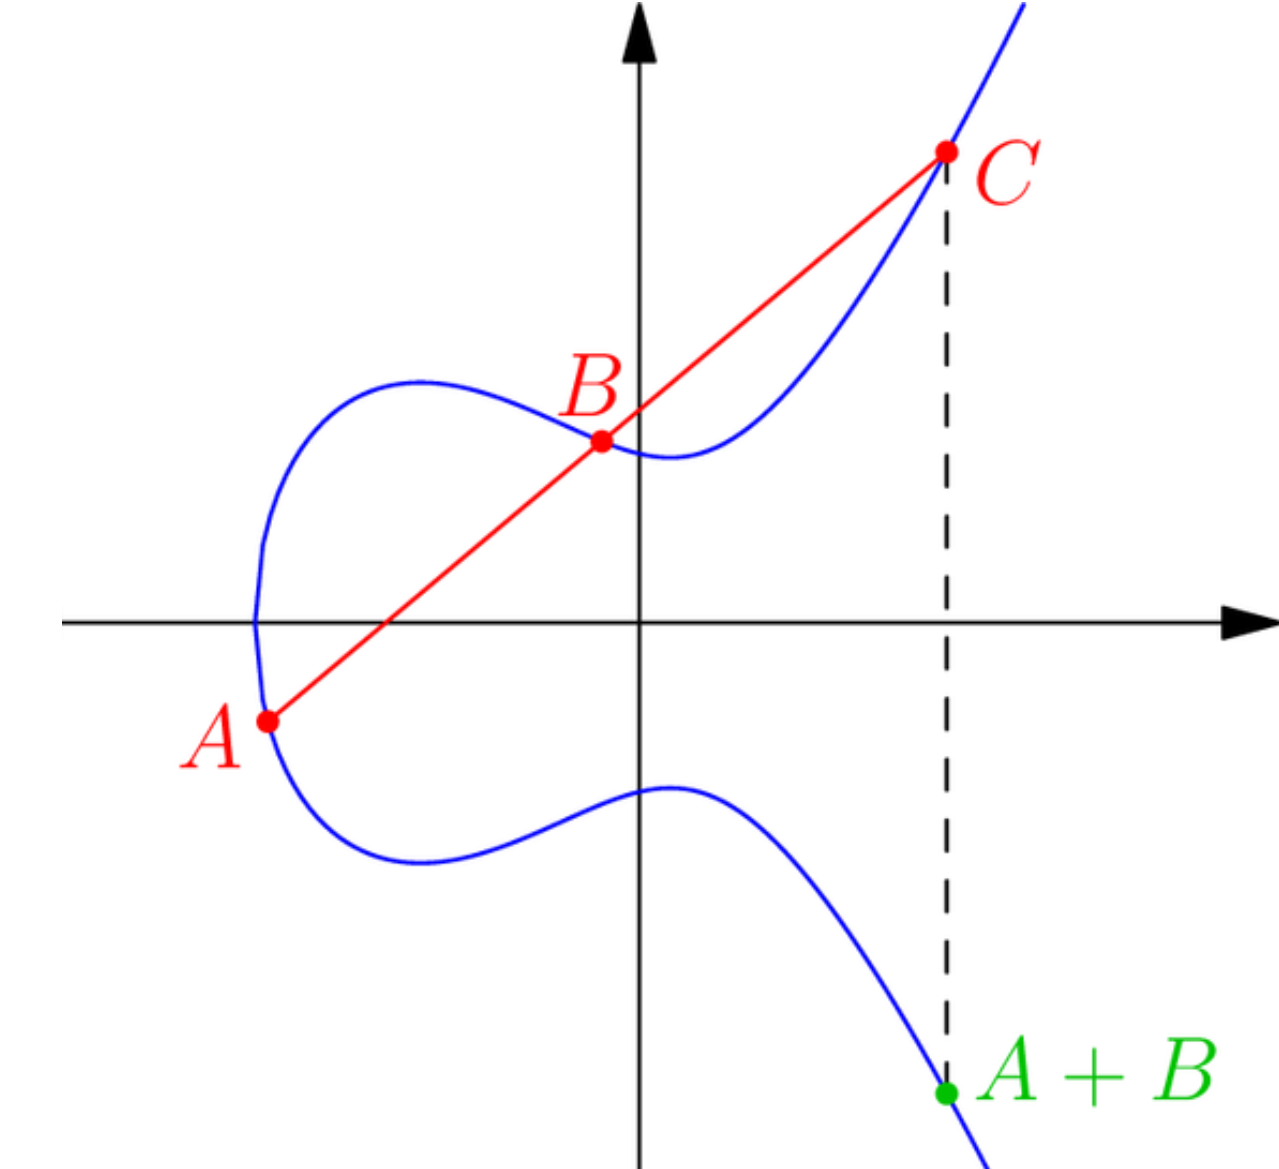
\includegraphics[angle=0,scale=0.4]{ECgrouplaw}
\end{figure}
\item More abstractly, one shows via Riemann--Roch that the map
\[P\mapsto (P)-(O) \in \textup{Div}^0(E/k)/\textup{lin. eq.}=\textup{Pic}^0(E/k)\]
is a bijection from $E(k)$ to $\textup{Pic}^0(E/k)$ with $O$ mapping to $0$. We can then pull back the group structure on $\textup{Pic}^0(E/k)$ to $E(k)$. 
\end{itemize}

These two ways are equivalent and turn out to give $E$ the structure of an \textit{abelian variety}. 

\begin{defi}
An $\textit{abelian variety}$ over $k$ is a nice group variety (i.e. a nice variety equipped with a group structure where the group operations are given by  morphisms).
\end{defi}

\begin{remark}
We have:
\begin{itemize}
\item The group structure is automatically abelian (this follows from projectivity). 
\item Any proper, connected, geometrically reduced group variety is in fact automatically smooth and projective, whence an abelian variety.
\item All one dimensional abelian varieties are elliptic curves (and, of course, conversely).
\item Over $\mathbb{C}$, any abelian variety of dimension $g$ is (as a complex Lie group) isomorphic to $\mathbb{C}^g/\Lambda$ for some lattice $\mathbb{Z}^{2g}\cong \Lambda\subseteq \mathbb{C}^g$.
\end{itemize}
\end{remark}


\subsection{Torsion points on abelian varieties}

Lots of current work in number theory is concerned with understanding as well as possible the group of rational points of abelian varieties over fields of arithmetic interest (e.g. number fields and their completions). Particularly accessible is the subgroup consisting of points of finite order. The following describes what the torsion points on an abelian variety look like over an algebraically closed field. Over $\mathbb{C}$ this follows from the last bullet point of the remark above.

\begin{theorem}
Let $k$ be a field  and $A/k$ an abelian variety of dimension $g$. Then for each $n\geq 1$ coprime to the characteristic of $k$ we have
\[A(\bar{k})[n]\cong (\mathbb{Z}/n\mathbb{Z})^{2g}.\]
%In particular, the natural $\textup{Gal}(\bar{k}/k)$ action on $A(\bar{k})[n]$ gives rise to a homomorphism
%\[\textup{Gal}(\bar{k}/k)\longrightarrow \textup{GL}\left(A(\bar{k})[n]\right)\cong GL_{2g}(\mathbb{Z}/n\mathbb{Z}).\]
\end{theorem}

It's often helpful to put all the torsion points (or all prime power torsion points for a fixed prime) together into an object called the \textit{Tate module}.

\begin{defi}[Tate module]
Let $k$ be a field, $A/k$ an abelian variety, and $l$ a prime number different from the characteristic of $k$. We define the $l$-adic Tate module $T_l(A)$ of $A$ to be the inverse limit
\[T_l(A)=\lim_{\leftarrow}A(\bar{k})[l^n].\]
As an abelian group this is abstractly isomoprhic to $\mathbb{Z}_l^{2g}.$
\end{defi}

\begin{remark}
For $n$ coprime to the characteristic of $k$, it turns out that all $n$-torsion points are contained in $A(k^\textup{sep})$. In particular, the absolute Galois group $\textup{G}_k$ of $k$ acts naturally on these points. In this way we get a $\mathbb{Z}_l$-linear action of $G_k$ on the $l$-adic Tate module $T_l(A)$, hence a $\mathbb{Q}_l$-linear action on 
\[V_l(A)=T_l(A)\otimes_{\mathbb{Z}_l}\mathbb{Q}_l.\]
We refer to this as the \textit{$l$-adic Galois representation associated to $A$}. %Fixing a basis for $V_l(A)$ induces a homomorphism 
%\[G_k\longrightarrow GL_{2g}(\mathbb{Q}_l)\]
%where $g$ is the dimension of $A$. This (at least conjecturally) encodes a huge amount of information about the abelian variety $A$.
\end{remark}

%\textbf{Dual abelian variety and autoduality of the Jaocbian?}

\subsection{Abelian varieties over number fields}

For this subsection we work over a number field $K$. Let $A/K$ be an abelian variety. The first starting point for understanding the group $A(K)$ is the Mordell--Weil theorem.

\begin{theorem}[Mordell--Weil theorem]
Let $K$ be a number field and $A/K$  an abelian variety. Then $A(K)$ is a finitely generated abelian group. Thus
\[A(K)\cong A(K)_{\textup{tors}}\oplus \mathbb{Z}^r\]
where $A(K)_{\textup{tors}}$ is a finite abelian group and $r\geq 0$ an integer. We call this integer $r$ the \emph{rank} of $A/K$, denoted $\textup{rk}(A/K)$.
\end{theorem}

The rank of an abelian variety is one of its most important invariants. It is, conjecturally, related via the Birch and Swinnerton--Dyer conjecture (see Maistret's course for more on this) to another important invariant: the $L$-function $L(A/K,s)$. 

\begin{defi}[The $L$-function of an abelian variety]
Let $A/K$ be an abelian variety of dimension $g$. For each nonarchimedean place $v$ of $K$ and prime $l$ with $v\nmid l$, we define the \textit{local L-polynomial}
\[L_v(A,T)=\det\left(1-\textup{Frob}_v^{-1}T|(V_l(A)^\vee)^{I_v}\right)\]
where here $I_v$ denotes the inertia group at $v$,  $\textup{Frob}_v$ is the (arithmetic) Frobenius at $v$, and $V_l(A)^{\vee}$ is the dual of $V_l(A)$. 

It's a general fact (which follows from the Weil conjectures and the existence of the N\'{e}ron model) that $L_v(A,T)$ is a polynomial with integer coefficients and is independent of the choice of $l$.  Writing $q_v$ for the size of the residue field at $v$, one defines the L\textit{-function} of $A/k$ to be the function of a complex variable $s$ given by
\[L(A/K,s)=\prod_{v\nmid \infty~\textup{place of }k}L_v(A,q_v^{-s})^{-1}.\]
\end{defi}

\begin{remark}
The $L$-function of any abelian variety can be shown to converge for $\textup{Re}(s)>3/2$ and conjecturally has analytic continuation to the whole of $\mathbb{C}$ satisfying a functional equation $s\leftrightarrow 2-s$. This is known for all elliptic curves over $\mathbb{Q}$ by work of Wiles, Taylor--Wiles, and Breuil--Conrad--Diamon--Taylor. More recently there has been much work towards this conjecture for elliptic curves over more general fields (totally real or CM) and for abelian surfaces over totally real fields. In particular, we now know analytic continuation for the $L$-function associated to an elliptic curve over totally real quadratic and cubic fields. oreover, we know meromorphic continuation for the $L$-function of an elliptic curve over all CM fields, and for the $L$-function of an abelian surface over totally real fields. See \cite{MR3359051},  \cite{DNS2019}, \cite{ACCGHLNSTT2018}, \cite{BCGP2018} and the references therein.
\end{remark}

\begin{example}
Let $E/K$ be an elliptic curve and $v$ a nonarchimedean place of $K$ of norm $q_v$. Let $\bar{E}/k_v$ be the reduction of a minimal Weierstrass equation at $v$, where $k_v$ is the residue field of $v$. If $E$ has good reduction at $v$ then  
\[L_v(E,T)=1-a_vT+q_vT^2\]
where $a_v=q_v+1-|\bar{E}(k_v)|$. For the places of bad reduction of $E$ we have
\[L_v(E,T)=\begin{cases}1-T~~&~~E\textup{ split mult at }v,\\ 
1+T~~&~~E\textup{ non-split mult at }v,\\ 1~~&~~ E\textup{ additive at }v.\end{cases}\]
\end{example}




\subsection{Jacobians}

The theory of curves and abelian varieties meets in \textit{Jacobians}, which are one of the main sources of examples of abelian varieties.

\begin{defi}[Approximate definition]
Let $C$ be a nice curve of genus $g$. Then one can naturally associate to $C$ a $g$-dimensional abelian variety $\textup{Jac}(C)$, the $\textit{Jacobian}$ of $C$, such that (as abelian groups) for any field extension $K/k$,
\[\textup{Jac}(C)(K)=\textup{Pic}^0\left(C/K^\textup{sep}\right)^{\textup{Gal}(K^\textup{sep}/K)}\]
functorially.
\end{defi}

\begin{remark} \label{actual defi remark}
More precisely, it's a theorem that the functor from $k$-schemes to abelian groups
\[T\mapsto \textup{Pic}^0\left(C_{T_{k^\textup{sep}}}\right)^{\textup{Gal}(k^\textup{sep}/k)}\]
is representable by an abelian variety over $k$. This representing object is the Jacobian of $C$.
\end{remark}

\begin{remark}
Since $\mathbb{P}^1_k$ has genus $0$ its Jacobian should be zero, which is reflected in the isomorphism $\textup{deg}:\textup{Pic}(\mathbb{P}^1_k)\stackrel{\sim}{\longrightarrow} \mathbb{Z}$ . Moreover, for an elliptic curve $E$, the Riemann--Roch argument shows that $E$ is its own Jacobian. 
\end{remark}

\begin{remark}
Let $C$ be a nice curve of genus $\geq 2$ with a $k$-point $O$. Then the Riemann--Roch argument generalises to give a closed immersion
$C\rightarrow \textup{Jac}(C)$ (induced by $P\mapsto (P)-(O)$)
called the \textit{Abel--Jacobi map}. If $k$ is a number field one of the main ways to understand the set $C(k)$ of rational points on $C$ is to attempt to understand the image of $C(k)$ inside its Jacobian.
\end{remark}

\begin{remark}
Even when the equation defining a curve is quite simple, the equations defining the Jacobian can be very complicated. For example, Flynn shows in \cite{MR1041476} that the Jacobian of a general genus $2$ curve $y^2=f(x)$ where $f(x)$ has degree $6$, is given by the vanishing of $72$ quadratic forms in $\mathbb{P}^{15}_k$ (over a field $k$ with $\textup{char}(k)\neq 2,3,5$). Consequently, one of our aims for this course is to describe how to compute certain invariants of Jacobians by working with the underlying curves. 
\end{remark}

\begin{remark}
We have a canonical isomorphism 
\[T_l(\textup{Jac}(C))\cong \textup{Hom}_{\mathbb{Z}_l}\left(H^1_{\textup{\'{e}t}}(C_{\bar{k}},\mathbb{Z}_l),\mathbb{Z}_l\right)\]
compatible with the Galois actions. Thus understanding the Tate module of the Jacobian of $C$ is the same as understanding the first \'{e}tale cohomology group of $C$.
\end{remark}

\subsection{The dual abelian variety}

One of the main things which distinguishes Jacobians from general abelian varieties is that they are canonically \textit{principally polarised}. To explain what this means we need to introduce the dual of an abelian variety. 

\begin{defi}[Approximate definition]
Let $A/k$ be an abelian variety. Then there is another abelian variety, $A^\vee/k$, of the same dimension of $A$, and such that, for any extension $K/k$, \[A^\vee(K)=\textup{Pic}^0\left(A/K\right)\]
functorially.\footnote{Here $\textup{Pic}^0(A/K)$ is the subgroup of $\textup{Pic}(A/K)$ consisting of line bundles algebraically equivalent to $0$. We do not need to  pass to a larger extension and  take galois invariants here since, unlike for curves, every abelian variety has at least one $k$-point.}  Again, this can be made precise in a way analagously to \Cref{actual defi remark}.
\end{defi}

Again, the Riemann--Roch argument shows that an elliptic curve is canonically isomorphic to its dual. The relavance of the dual abelian variety for arithmetic is that a lot of natural pairings (the Weil pairing, local duality pairings, the Cassels--Tate pairing,...) naturally take place not between an abelian variety and itself, as is the case for elliptic curves, but between an abelian variety and its dual. However, abelian varieties are closely related to their duals via the notion of a polarisation. 

\begin{defi}
Let $\mathcal{L}$ be a line bundle on an abelian variety $A/k$ and $x\in A(k)$. Writing $\tau_x$ for the `translation-by-$x$' morphism, the line bundle 
\[\tau^*_x\mathcal{L}\otimes \mathcal{L}^{-1}\]
is algebraically equivalent to zero. This construction gives a map $A(k)\rightarrow A^\vee(k)$, 
\[x \longmapsto \tau^*_x\mathcal{L}\otimes \mathcal{L}^{-1}.\]
 In fact, this can be ramped up to give a homomorphism of abelian varieties 
\[\phi_\mathcal{L}:A\longrightarrow A^\vee.\]
In general, any homomorphism $A\rightarrow A^\vee$ which arises via this construction after base-extension to $\bar{k}$ is called a \textit{polarisation}.
A polarisation is called \textit{principal} if it's an isomorphism.
\end{defi}  

\begin{remark}
One can show that a polarisation is an \textit{isogeny} (finite kernel in this context) if and only if the line bundle $\mathcal{L}$ is ample.  
Since all abelian varieties are projective they come endowed with at least one (very) ample line bundle, and are thus always isogeneous to their duals. This has a number of consequences for their arithmetic. For example, over a number field an abelian variety has the same rank and $L$-function as its dual.
\end{remark}

\begin{proposition}
Let $C/k$ be a nice curve. Then $J=\textup{Jac}(C/k)$ is canonically principally polarised. 
\end{proposition}

\begin{proof}[Sketch of proof]
We'll first do this over $\bar{k}$. Pick an initial point $O\in C(\bar{k})$. For any $n$, we have a morphism (defined over $\bar{k}$) $C^n\rightarrow J$ induced by
\[(P_1,...,P_n)\mapsto \sum_{i=1}^n (P_i) - n(O).\]
It turns out that when $n=g-1$ the image is an effective divisor on $J$, and hence yields a line bundle $\Theta$ on $J$ called the \textit{Theta bundle}. The resulting polarisation $\phi_\Theta:J\rightarrow J^\vee$ can be shown to be principal, and does not, in fact, depend on the choice of initial point $O$. Using this latter fact, one can additionally show that the morphism $\phi_{\Theta}$ (although not $\Theta$ in general) is defined over $k$.
\end{proof}

\newpage

\section{Exercises for lecture 1}


\subsection{}
Let $k$ be an algebraically closed field of characteristic different from $2$, and let $C:y^2=f(x)$ be a hyperelliptic curve over $k$ of genus $g\geq 2$. Suppose that $f(x)$ has odd degree $2g+1$ and denote by $\mathcal{R}$ the set of roots of $f(x)$.
\begin{itemize}
\item[(i)] Show that the ramification points of the $x$-coordinate map $\phi:C\rightarrow \mathbb{P}^1$ are the points $P_r=(r,0)$ for $r\in \mathcal{R}$, along with the unique point $O$ at infinity.
\item[(ii)] Show that each of the degree $0$ divisors \[\{(P_r)-(O)~~\mid ~~r\in \mathcal{R}\}\] are $2$-torsion points in the Jacobian of $C$.
\item[(iii)] Show that, for $k$ now not necessarily algebraically closed, as a $\textup{G}_k$-module, the $2$-torsion subgroup of the Jacobian of $C$ is isomorphic to
\[\mathbb{F}_2[\mathcal{R}]/\Sigma\]
where $\mathbb{F}_2[\mathcal{R}]$ denotes the permuation module on $\mathcal{R}$ with $\mathbb{F}_2$-coefficients, and $\Sigma$ is the formal sum of  the elements of $\mathcal{R}$. 
\item[(iv)] What is the analagous description in the case where $f(x)$ has even degree?
\end{itemize}

\subsection{}
Let $k$ be an algebraically closed field of characteristic different from $2$, and let $C:y^2=f(x)$ be a hyperelliptic curve over $k$ of genus $2$ (so that $f$ has degree 5 or 6). Denote by $\iota$ the \textit{hyperelliptic involution} sending a point $P=(x,y)$ to $(x,-y)$. 
\begin{itemize}
\item[(i)] Show that the class of the canonical divisor $K_C$ is represented by the divisor $P+\iota(P)$ for any point $P$ on $C$ (hint: consider the degree $2$ map to $\mathbb{P}^1$ and use Riemann--Hurwitz).
\item[(ii)] Show that the map sending  $\{P_1,P_2\}$  to the divisor $(P_1)+(P_2)-(O)-(\iota(O))$ (for $O$ any point at infinity) is a surjection from the set of unordered pairs of points on $C$, to the set degree $0$ divisors on $C$ modulo linear equivalence. Show that the inverse image of any degree $0$ divisor class other than $0$ consists of a unique pair. What is the inverse image of the $0$ class? (Note that for a general (say perfect) field $k$ this gives a description of $\textup{Jac}(C)(\bar{k})$ as a $G_k$-set.)
\item[(iii)*] How would one go about adding two points $\{P_1,P_2\}$ and $\{Q_1,Q_2\}$ of $\textup{Jac}(C)$ via this identification?
\end{itemize}

\newpage

\section{Models of curves and abelian varieties}

In order to understand the behaviour of curves and abelian varieties over number fields it's natural to first try to understand them over completions of number fields. In particular the $L$-function, for example, is defined only using the abelian variety over all completions. Thus we now move from arbitrary fields to a fixed finite extension $K$ of $\mathbb{Q}_p$ for a prime $p$ (of course, there is also a lot of interesting stuff going on over the real numbers and the complex numbers, but we will not persue this further). Let $\mathcal{O}_K$ denote the ring of integers of $K$, and $k$ the residue field. Our general philosophy is to study  curves and Jacobians over $K$ by reducing, as much as possible, to questions over the finite field $k$. This can often reduce questions to a finite computation, whilst from a theoretical point of view the Weil conjectures give a huge  tool to draw on. The key method for moving from $K$ to its residue field is given by the theory of models. Roughly, the idea is that one wants to `reduce modulo $p$' but before one can do this the equations defining the variety in question need to have coefficients in $\mathcal{O}_K$. Of course, there are many changes of variables over $K$ which achieve this and we need to single out ones which are particularly useful.

\subsection{Motivation: elliptic curves}

Let $p$ be a prime taken, for simplicity, not equal to $2,3$ and let \[E/\mathbb{Q}_p:y^2=x^3+ax+b\] be an elliptic curve. After a change of variable of the form $(x,y)\mapsto (u^2x,u^3y)$ for $u\in \mathbb{Q}_p^\times$ we can assume that $a,b\in \mathbb{Z}_p$ and that $\textup{ord}_p(\Delta_E)$ is minimal amongst all such equations. We call this the \textit{minimal Weierstrass equation} for $E$. The reduction modulo $p$, 
\[\bar{E}/\mathbb{F}_p:y^2=x^3+\bar{a}x+\bar{b},\]
is well defined (up to isomorphism over $\mathbb{F}_p$) and falls into one of three cases:
\begin{itemize}
\item $\bar{E}/\mathbb{F}_p$ is an elliptic curve. This happens if and only if $\textup{ord}_p(\Delta_E)=0$ and is referred to as \textit{good reduction}.
\item $\bar{E}/\mathbb{F}_p$ has a node. This happens if the polynomial $x^3+ax+b~~\textup{(mod }p)$ has a unique double root and is referred to as \textit{multiplicative reduction}.
\item $\bar{E}/\mathbb{F}_p$ has a cusp. This happens if the polynomial $x^3+ax+b~~\textup{(mod }p)$ has a triple root and is referred to as \textit{additive reduction}.
\end{itemize}
Moreover, the subset of non-singular points on $\bar{E}$ have a natural group structure. 

\begin{remark}
If $E$ has good reduction then it does so over any extension of $\mathbb{Q}_p$ also, and the same is true of multiplicative reduction. On the other hand, additive reduction becomes either good or multiplicative after a finite extension. In fact, as $p\neq 2$, any ramified quadratic extension of the splitting field of $x^3+ax+b$ suffices.
\end{remark}

For general curves $C/\mathbb{Q}_p$ we have a similar picture to the one above, but we need some more involved theory to describe it. 

\subsection{Models of curves}

As before, let $K$ be a finite extension of $\mathbb{Q}_p$, $\mathcal{O}_K$ its ring of integers and $k$ its residue field. Fix a nice curve $C/K$. 

\begin{defi}
A \textit{model} of $C$ is a scheme $\mathcal{C}/\mathcal{O}_K$, finite type, flat and proper\footnote{Roughly, flatness ensures that the resulting reduction retains information about $C$ (such as being connected, having dimension $1$, having arithmetic genus equal to the genus of $C$) and properness ensures projectivity of the reduction and the existence of a reduction map on points.} over $\mathcal{O}_K$, and equipped with a specified isomorphism \[\mathcal{C}\times_{\mathcal{O}_K}K\stackrel{\sim}{\longrightarrow} C\] of schemes over $K$. We refer to $\mathcal{C}\times_{\mathcal{O}_K}K$ as the \textit{generic fibre} of $\mathcal{C}$, and define its \textit{special fibre} to be the $k$-scheme
\[\overline{\mathcal{C}}=\mathcal{C}\times_{\mathcal{O}_K}k.\]
\end{defi} 

The picture is as follows (genera added to illustrate how arithmetic genus is presrved when passing to the special fibre):

\begin{figure} [!htb] 
%\caption{Special fibre and dual graph}
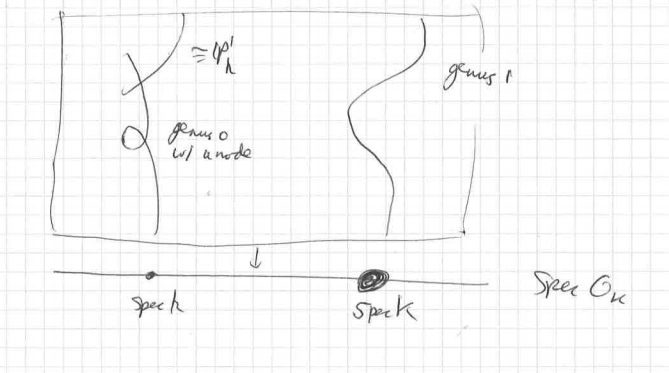
\includegraphics[angle=0,scale=0.6]{model}
\end{figure}

\begin{example}
Let $E/\mathbb{Q}_p$ be an elliptic curve say with minimal Weierstrass equation $E:y^2=x^3+ax+b$, $a,b\in \mathbb{Z}_p$. Then we can consider the scheme
\[\mathcal{E}:\{y^2z-x^3-axz^2-bz^3=0\}\subseteq \mathbb{P}^2_{\mathbb{Z}_p}\]
which is a model of $E$. Its special fibre is the curve $\bar{E}$ above (along with the usual point at infinity). We will refer to this as the \textit{minimal Weierstrass model}. 
\end{example}

For elliptic curves the minimal Weierstrass model gives a `best' model of $E$ over $\mathbb{Z}_p$. In some sense, it's the model which gives the special fibre the best chance of being an elliptic curve over $\mathbb{F}_p$. In general, we want to find an equation free method for specifying a `best' or a least `not that bad' model of a curve. 

There are, broadly, two ways to go:

\begin{itemize}
\item Insist that the scheme $\mathcal{C}/\mathcal{O}_K$ is regular (`smooth as a surface').
\item Ask that the special fibre be `not too bad'. The usual thing to ask for is that it be `semistable' (the analogue of the special fibres of good or multiplicative elliptic curves).
\end{itemize}

The first of these is always possible and in fact there is a minimal such model (assuming that $C$ has genus at least $1$), the \textit{minimal regular model}\footnote{Formally, we say a regular model $\mathcal{C}$ for $C$ is \textit{minimal} if for every other regular model $\mathcal{C}'$ for $C$, the map between their generic fibres corresponding to the identity  on $C$ extends to a morphism $\mathcal{C}'\rightarrow \mathcal{C}$. One can show that there always exists a regular model of $C$ that is minimal in this sense, which is necessarily unique. This is the \textit{minimal regular model} of $C$.}. This is a fundamental object however the special fibres of these models can still be quite complicated. By contrast, semistable curves (to be discussed shortly) are all quite simple, however it is not always the case that a given curve has a semistable model. That said,  one can always find one over a finite extension of $K$ in which case there is a minimal such (now assuming that $C$ has genus at least $2$). Moreover, when such a model can be found the minimal regular model has semistable special fibre also. We will focus on semistable curves, as they are easier to work with and are all that is needed for many problems. However, there are still cases when one needs to work with a regular model instead and computing (with) these models is an important topic which we will not discuss further.

The best possible situation, which is an instance of both cases above, is when the special fibre is in fact a nice curve. Indeed, nice curves are in particular semistable and when the special fibre is a nice curve the structure map $\mathcal{C}\rightarrow \textup{Spec}\mathcal{O}_K$ is smooth whence  $\mathcal{C}$ is regular. 

\begin{defi}
We say that $C$ has \textit{good reduction} if there is a model $\mathcal{C}$ of $C$ whose special fibre is a nice curve over $k$.
\end{defi}

\begin{example}
Note that:

\begin{itemize} 
\item If $E$ is an elliptic curve then this is consistent with what we had previously (at least, if an elliptic curve has good reduction in the first sense, then it also has good reduction in the second; the converse is also true but not immediately obvious). 
\item Suppose $C:y^2=f(x)$ is a hyperelliptic curve over $\mathbb{Q}_p$, $p\neq 2$, and suppose that $f(x)\in \mathbb{Z}_p[x]$ is such that $\textup{ord}_p(\Delta(f))=0$ where $\Delta(f)$ is the discriminant of $f(x)$. Then we may glue the affine schemes
\[\mathcal{U}_1=\textup{Spec}\mathbb{Z}_p[x,y]/(y^2-f(x))\]
and
\[\mathcal{U}_2=\textup{Spec}\mathbb{Z}_p[w,z]/(z^2-w^{2g+2}f(1/w))\]
along $x=1/w$ and $y=w^{g+1}z$ over the open subsets $x\neq 0$ and $x\neq 0$ respectively. The resulting scheme is a model of $C$ whose special fibre is the nice hyperelliptic curve given by the equation $y^2=\bar{f}(x)$, where $\bar{f}(x)$ is the reduction of $f(x)$ modulo $p$.    
\end{itemize}
\end{example}

\begin{remark} 
One can show that if $C$ has genus at least $1$ and $\mathcal{C}$ and $\mathcal{C}'$ are models of $C$ with good reduction, then (as follows from the existence of the minimal regular model)  $\mathcal{C}$ and $\mathcal{C}'$ are isomorphic over $\mathbb{Z}_p$. 
\end{remark}


\subsection{The structure of singular curves}

The aim of this subsection is to motivate and define semistable curves, and study their properties. To begin with suppose $k=\bar{k}$ and let $X$ be a projective, reduced, connected curve (possibly singular and with multiple irreducible components). Denote by $X_\textup{sing}$ the set of singular points of $X$.

\begin{defi}
The \textit{normalisation} of $X$, $\tilde{X}$, is the disjoint union of the normalisations of the individual components (and is thus a disjoint union of nice curves). It comes with a natural morphism $\pi:\tilde{X}\rightarrow X$ which is an isomorphism away from $X_\textup{sing}$. 
\end{defi}


The picture is as follows:

\begin{figure} [!htb] 
%\caption{Special fibre and dual graph}
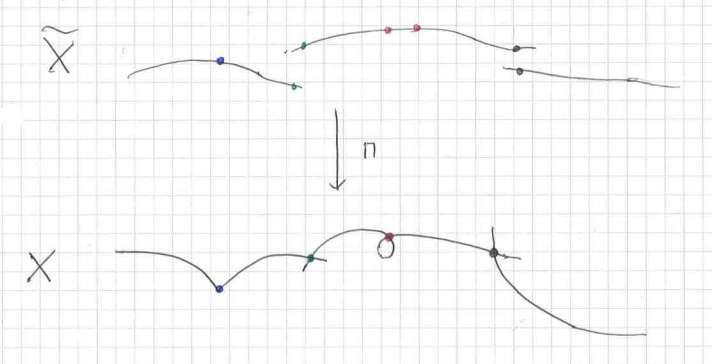
\includegraphics[angle=0,scale=0.5]{normalisation}
\end{figure}

\begin{remark}
Locally in some affine $U=\textup{Spec}(A)\subseteq X$, the irreducible components which intersect $U$ correspond to the minimal prime ideals $\mathfrak{p}_1,...,\mathfrak{p}_r$ of $A$. Then $\tilde{U}=\pi^{-1}(U)$ is
\[\textup{Spec}\left(\prod_{i=1}^r \widetilde{A/\mathfrak{p}_i}\right),\]
where $\widetilde{A/\mathfrak{p}_i}$ is the integral closure of $A/\mathfrak{p}_i$ in its field of fractions. The morphism $\pi$ is  given by the natural inclusion of $A$ into the direct product.
\end{remark}

To measure `how singular' $X$ is, we measure the difference between $X$ and its normalisation $\tilde{X}$. This is done by considering the short exact sequence of sheaves
\begin{equation} \label{first sheaf seq}
0\longrightarrow \mathcal{O}_X\longrightarrow \pi_*\mathcal{O}_{\tilde{X}}\longrightarrow \mathcal{S}\longrightarrow 0
\end{equation}
with $\mathcal{S}$ defined by the sequence. Since $\pi$ is an isomorphism away from $X_\textup{sing}$ it's a skyscraper sheaf supported on $X_\textup{sing}$. 

\begin{defi}
For $x\in X$ a closed point, we define
\[\delta_x:=\textup{dim}_k \mathcal{S}_x=\textup{dim}_k \widetilde{\mathcal{O}_{X,x}}/\mathcal{O}_{X,x}\]
where here $\widetilde{\mathcal{O}_{X,x}}$ is the product of the normalisations of $\mathcal{O}_{X,x}/\mathfrak{p}_i$ where the $\mathfrak{p}_i$ are the minimal prime ideals of $\mathcal{O}_{X,x}$; they correspond to the irreducible components of $X$ passing through $x$.
We note that $x$ is smooth if and only if $\delta_x=0$. We also define $m_x:=\#\pi^{-1}(x)$. We say that $x$ is a \textit{ordinary double point}, or a \textit{node}, if $m_x=2$ and $\delta_x=1$.
\end{defi}

\begin{remark}
One can show that $x\in X$ is an ordinary double point if and only if the completed local ring at $x$ is isomorphic to $k[[u,v]]/(uv)$. That is, the completed local ring is isomorphic to the completed local ring at the origin of the curve given by the two coordinate axes in $\mathbb{A}^2$. This is the picture of what an ordinary double point looks like to have in mind. 
\end{remark}

\begin{example}[Plane curves] \label{plane curve example}
Let $X$ be an affine plane curve given by an equation $\{f(x,y)=0\}\subseteq \mathbb{A}^2$ and suppose that $(0,0)\in X$. Then we can write 
\[f(x,y)=a_1x+a_2y+b_1x^2+b_2xy+b_3y^2+...\]
Then $(0,0)$ is a singular point of $X$ if and only if $a_1=0=a_2$, and an ordinary double point if and only if the discriminant
\[b_2^2-4b_1bb_3\]
of the quadratic term is non-zero. 
\end{example}


\begin{remark}
The structure of a singular point is a local property  so if $x\in X$ has an open neighbourhood isomorphic to an open neighbourhood of a plane curve then we can still use the above example.
\end{remark}

\begin{defi}
We say that $X$ is \textit{semistable} if (it is reduced and) all its singular points are ordinary double points. If $k$ is no longer assumed algebraically closed, we say that a curve $X/k$ is \textit{semistable} if $X$ if $X_{\bar{k}}$ is semistable.
\end{defi}

\begin{example}
If $E/\mathbb{Q}_p$ is an elliptic curve, and $\bar{E}/\mathbb{F}_p$ is the reduction of its minimal Weierstrass equation, then the example above shows that $\bar{E}$ is semistable if and only if $E$ has good or multiplicative reduction.
\end{example}

\begin{example}
Let $C:y^2=f(x)$ be a possibly singular `hyperelliptic' curve over $k$ where $\textup{deg}(f)>2$ and $\textup{char}(k)\neq 2$. Then $C$ is semistable if and only if $f(x)$ has no roots of multiplicity higher than $2$.
\end{example}

A slight refinement of the notion of a semistable curve is a stable curve. 

\begin{defi}[Stable curves]
If $k=\bar{k}$, we say that $X$ is \textit{stable} if it is semistable and if $X$ has arithmetic genus at least $2$, and any irreducible component of $X$ isomorphic to $\mathbb{P}^1_k$ intersects the other irreducible components in a least $3$ points. For general $k$, we say that $X$ is stable if $X_{\bar{k}}$ is.
\end{defi}

%The difference is shown in the picture below. 
%
%\begin{figure} [!htb] 
%%\caption{Special fibre and dual graph}
%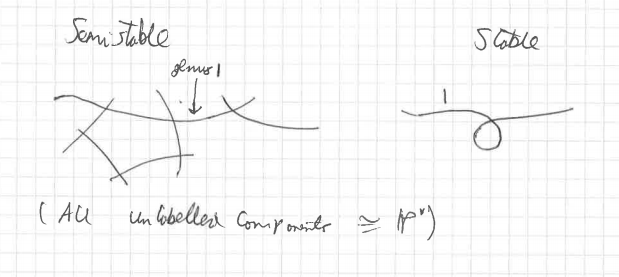
\includegraphics[angle=0,scale=0.6]{stable}
%\end{figure}

\begin{remark} 
Equivalently, a semistable curve over an algebraically closed field is stable if and only if its automorphism group is finite.
\end{remark}

\subsection{The dual graph of a semistable curve}

A useful invariant of a semistable curve (as we will see later) is its dual graph, which is defined as follows.

\begin{defi}[Dual graph]
Let $k=\bar{k}$ and $X$ be a semistable curve over $k$. We define the \textit{dual graph} of $X$ to be the graph whose vertices are the irreducible components of $X$, and such that vertices $v_1$ and $v_2$ (where $v_1=v_2$ is allowed) are joined by one edge for each singular point lying on both of the corresponding irreducible components. Note that loops and multiple edges are allowed.
\end{defi}

\begin{example} \label{dual graph ex 1}
Suppose $\textup{char}(k)\neq 2$ and consider the singular hyperelliptic curve 
\[y^2=x^2(x-1)^2(x+1)^2.\]
This consists of two irreducible components intersecting in $3$ (ordinary double) points. 
\begin{figure} [!htb] 
%\caption{Special fibre and dual graph}
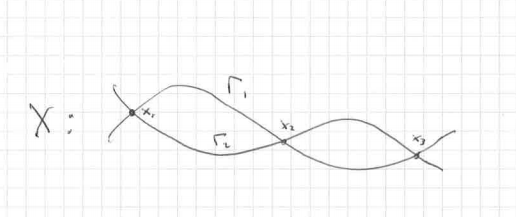
\includegraphics[angle=0,scale=0.5]{curve_1}
\end{figure}

Its dual graph is the `banana graph':

\begin{figure} [!htb] 
%\caption{Special fibre and dual graph}
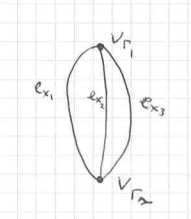
\includegraphics[angle=0,scale=0.6]{dual_graph_1}
\end{figure}
\end{example}

\begin{example} \label{dual graph ex 2}
Suppose now that $\textup{char}(k)\neq 2,3$ and consider the singular hyperelliptic curve
\[y^2=x^2(x-1)^2(x+1)^2(x-2).\]
Now this consists of one irreducible component with $3$ nodes on it.
\begin{figure} [!htb] 
%\caption{Special fibre and dual graph}
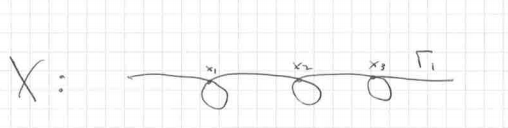
\includegraphics[angle=0,scale=0.7]{curve_2}
\end{figure}

Its dual graph is:

\newpage

\begin{figure} [!htb] 
%\caption{Special fibre and dual graph}
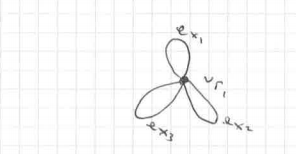
\includegraphics[angle=0,scale=0.8]{dual_graph_3}
\end{figure}
\end{example}

%\begin{remark} \label{semistable arithmetic genus}
%We'll see lots of uses for the dual graph in the next two lectures. However, as a first indication of the utility of this notion, we note that (with $k=\bar{k}$), the arithmetic genus of a semistable curve $X$ is equal to the sum of the genera of the normalisations of its irreducible components, plus the rank of the first homology group of the graph:
%\[p_a(X)=\sum_{\Gamma\textup{ irred. comp of }X}g(\Gamma)+E(\mathcal{G})-V(\mathcal{G})+1\]
%where here $g(\Gamma)$ is the geometric genus of an irreducible component, $E(G)$ is the number of edges in the dual graph $\mathcal{G}$, and $V(\mathcal{G})$ the number of vertices. 
%\end{remark}

\subsection{Semistable models}

We now return to the case where $K$ is a finite extension of $\mathbb{Q}_p$ and $C/K$ is a nice curve. We say $C$ has \textit{semistable reduction} over $K$ if there is a model $\mathcal{C}/\mathcal{O}_K$ for $C$ whose special fibre is a semistable curve over the residue field $k$. We call such a model a \textit{semistable model} for $C$. If additionally the special fibre of $\mathcal{C}$ is stable we call this a \textit{stable model}.

Whilst it's not true that all curves admit semistable models (cf. elliptic curves with additive reduction) the power of the theory of semistable models lies in the following deep result of Deligne--Mumford.

\begin{theorem}[Semistable reduction theorem]
Let $C/K$ be a nice curve. Then there is a finite extension $L/K$ such that $C$ has semistable reduction over $K$.
\end{theorem}

A slight refinement which follows fairly quickly from this is:

\begin{proposition} 
Let $C/K$ be a nice curve of genus at least $2$ and $L/K$ any finite extension where $C$ has semistable reduction. Then $C$ has a stable model $\mathcal{C}$ over $\mathcal{O}_L$ which is unique up to $\mathcal{O}_L$-isomorphism. Moreover, if $F/L$ is a further finite extension, then $\mathcal{C}\times_{\mathcal{O}_L}\mathcal{O}_F$ is the stable model of $C$ over $F$.
\end{proposition}

In particular, we can talk about \textit{the} stable reduction of $C$.

\subsection{Relationship between the stable model and the minimal regular model}

In general, if ($K$ is a finite extension of $\mathbb{Q}_p$ and) $C/K$ is a semistable curve,  its minimal regular model is readily obtained from its stable model by some simple blow ups. To explain this, let $\mathcal{C}/\mathcal{O}_K$ be the stable model of $C$. If a closed point $x\in \mathcal{C}$ is non-regular then it is necessarily a singular point of the special fibre, and hence corresponds to an ordinary double point on the special fibre $\bar{\mathcal{C}}$. If we assume that both $x$ and the two points lying over $x$ in the normalisation of $\bar{\mathcal{C}}$ are defined over $k$, it follows formally from the fact that the completed local ring at $x\in  \bar{\mathcal{C}}$ is isomorphic to $k[[u,v]]/(uv)$, that the completed local ring at $x\in \mathcal{C}$ is isomorphic to $\mathcal{O}_K[[u,v]]/(uv-c)$ for some $c\in \mathcal{O}_K$ of valuation $\geq 1$. The valuation of $c$, say $n$, is called the \textit{thickness} of the ordinary double point. One sees that $x$ is a regular point of $\mathcal{C}$ if and only if $n=1$. When $n> 1$ one can repeatedly blow up at $x$ to resolve the singularity. If this is done minimally, the result is given by replacing $x$ by  a chain of $n-1$ copies of the projective line, each intersecting transversally. See \cite[Corollary 10.3.25]{MR1917232} and the surrounding discussion for more details. The picture is as follows: 

\begin{figure} [!htb] 
%\caption{Special fibre and dual graph}
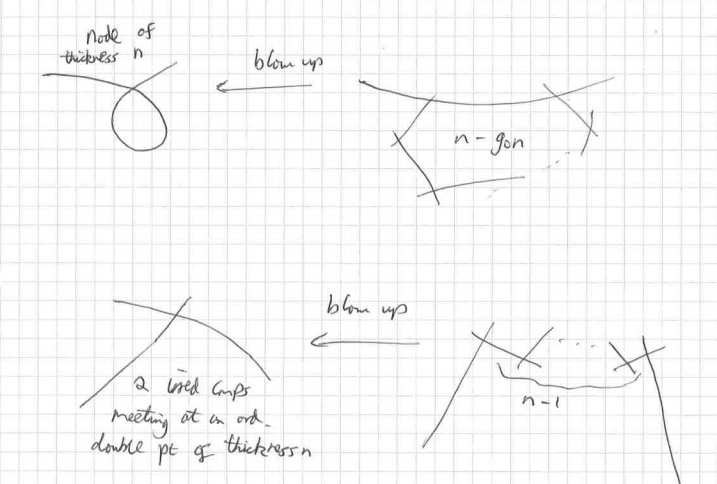
\includegraphics[angle=0,scale=0.5]{thickness}
\end{figure}



\newpage 


In general, the condition that $x$ and the points over it in the normalisation be defined over $k$ is always satisfied after finite extension of $k$. If one then follows the above procedure  at every ordinary double point of $\bar{\mathcal{C}}$ this yields the minimal regular model of $C/K$.  Since the minimal regular model commutes with unramified extension, we can always make an unramified extension of $K$ to make this true. As a corollary we find:

\begin{cor}
If $C/K$ has semistable reduction its minimal regular model is a semistable model for $C$.
\end{cor} 

\newpage

\section{Exercises for lecture 2}


\subsection{}
Justify \Cref{plane curve example}: let $X$ be an affine plane curve over an algebraically closed field $k$, given by an equation $\{f(x,y)=0\}\subseteq \mathbb{A}^2$ and suppose that $(0,0)\in X$. Write 
\[f(x,y)=a_1x+a_2y+b_1x^2+b_2xy+b_3y^2+...\]
Show that $(0,0)$ is a singular point of $X$ if and only if $a_1=0=a_2$. Supposing $(0,0)$ is singular, compute the completed local ring at $(0,0)$ in the case that the discriminant
\[b_2^2-4b_1b_3\]
of the quadratic term is non-zero, and deduce that $(0,0)$ is an ordinary double point. 

\subsection{}
Let $k$ be an algebraically closed field. The \textit{aritmetic genus} $p_a(X)$ of a (projective, reduced, connected) curve $X/k$ is defined to be the $k$-dimension of $H^1(X,\mathcal{O}_X)$. Show that if $X$ is semistable then 
\[p_a(X)=\#\textup{edges of }\mathcal{G}-\# \textup{vertices of }\mathcal{G}+1+\sum_{\Gamma \textup{ irred comp of }X} g(\tilde{\Gamma})\]
where $\mathcal{G}$ is the dual graph of $X$, and $g(\tilde{\Gamma})$ denotes the  genus of the normalisation of $\Gamma$. 

(One can rewrite the sum $\#\textup{edges of }\mathcal{G}-\# \textup{vertices of }\mathcal{G}+1$ as the rank of the first homology group
$H_1(\mathcal{G},\mathbb{Z})$ of $\mathcal{G}$.)

\subsection{}
Let $p$ be odd and $C/\mathbb{Q}_p:y^2=f(x)$ be a hyperelliptic curve where $f(x)$ is monic and has coefficients in $\mathbb{Z}_p$. Suppose that the discriminant of $f(x)$ has $p$-adic valuation $1$. Show that the scheme over $\mathbb{Z}_p$ given by glueing the usual charts
\[\textup{Spec }\mathbb{Z}_p[x,y]/(y^2-f(x))\]
and
\[\textup{Spec }\mathbb{Z}_p[w,z]/(z^2-w^{2g+2}f(1/w))\] 
via $x=1/w$ and $y=w^{g+1}z$ gives both a regular\footnote{By definition, a scheme $X$ is regular if for each $x\in X$ the  local ring $\mathcal{O}_{X,x}$ at $x$ is regular, i.e. if its dimension is equal to the $\mathcal{O}_{X,x}/\mathfrak{m}_x$-dimension of $\mathfrak{m}_x/\mathfrak{m}_{x}^2$, where $\mathfrak{m}_x$ is the maximal ideal of $\mathcal{O}_{X,x}$. To check regularity it suffices to check this for $x$ a closed point.} and semistable model of $C$ (in particular, this is the minimal regular model of $C$).

\newpage

\section{Lecture 3: Semistable models of hyperelliptic curves and N\'{e}ron models of abelian varieties}

\subsection{Semistable models of hyperelliptic curves: introduction}

Again, $K$ is a finite extension of $\mathbb{Q}_p$, ring of integers $\mathcal{O}_K$, residue field $k$. The aim of this lecture is to give some examples of computing the (potential) stable reduction of curves. Our examples will come from hyperelliptic curves over finite extensions of $\mathbb{Q}_p$ with $p$ odd. We will just state the results rather than giving proofs, but the idea is as follows. By definition a hyperelliptic curve comes equipped with a degree $2$ morphism $\phi:C\rightarrow \mathbb{P}^1_K$. Let $B$ be the branch locus of this morphism, i.e. the points of $\mathbb{P}^1_K$ above which this map ramifies. If $C$ is given by an equation $y^2=f(x)$ then the map $\phi$ is projection to the $x$ coordinate and $B$ is the collection of roots of $f(x)$, along with the point at infinity if $f(x)$ has odd degree. The scheme $\mathbb{P}^1_{\mathcal{O}_K}$ gives a regular proper semistable model of $\mathbb{P}^1_K$. Taking the closure of $B$ in $\mathbb{P}^1_{\mathcal{O}_K}$ gives a divisor on $\mathbb{P}^1_{\mathcal{O}_K}$. The idea is to blow up at closed points on the special fibre of $\mathbb{P}^1_{\mathcal{O}_K}$ to gradually improve this divisor. At any stage of this process we may take the normalisation of the resulting  model of $\mathbb{P}^1_K$ in $K(C)$. This will give a model of $C$ and, if the new divisor is sufficiently nice, will be regular/semistable/stable (of course, the last two will in general need an extension of $K$).

 This approach works more generally to produce (potential) stable models of cyclic covers of the projective line (for residue characteristic different from the degree of the cover) and has been described algorithmically for superelliptic curves by Bouw--Wewers in \cite{MR3576328}. See https://pypi.org/project/mclf/ for a sage implementation in certain cases. The particular framework described below is set out in \cite{M2D2}, although we make several simplyfying assumptions.
 
 \subsection{Setup}

Take $p$ to be odd. Let $\pi_K$ be a uniformiser for $K$ and denote by $v:K^\times \rightarrow \mathbb{Z}$ the normalised valuation. Let $C:y^2=f(x)$ be a hyperelliptic curve over $K$ of genus $g\geq 2$, so that $f(x)$ is a squarefree polynomial of degree at least $5$. We will describe the stable model of $C$ (possibly over an extension of $K$) by describing both the dual graph, and the normalisation of each irreducible component, of its special fibre. The answer will be in terms of the combinatorial data set out below.

\subsection{Clusters}

Denote by $\mathcal{R}$ the set of roots of $f(x)$, and $c_f$ the leading coefficient of $f(x)$, so that $C$ has equation
\[C:y^2=c_f\prod_{r\in \mathcal{R}}(x-r).\] 

\begin{assumption}
We assume:
\begin{enumerate}
 \item  The set of roots $\mathcal{R}$ is contained in $K$. If this is not the case we simply replace $K$ by a finite extension for which this does hold. 
 \item We assume that $|\mathcal{R}|=2g+1$. Given (1) this can be achieved by a change of variables sending a point $(r,0)$ ($r$ a root of $f(x)$) to infinity. 
 \end{enumerate}
\end{assumption}

\begin{defi}
A \textit{cluster} is a nonempty subset of $\mathcal{R}$ cut out by a disc. That is, a nonempty subset of the form
\[\mathfrak{s}=\{r\in \mathcal{R}~~\mid~~ v(r-z)\geq n\}\]
for some $z\in K$ and $n\in \mathbb{Z}$ (note that if we wish we can without loss of generality take $z$ to be a root of $f(x)$). If $\mathfrak{s}$ is a cluster of size at least $2$ then amongst all such pairs $(z,n)$ `cutting out' $\mathfrak{s}$, the maximal $n$ is called the \textit{depth} of $\mathfrak{s}$, denoted $d_{\mathfrak{s}}$. 
\end{defi}

Note that $\mathcal{R}$ and each singleton $\{r\}$ for $r\in \mathcal{R}$ are clusters. 

\begin{example} \label{cluster example}
Consider the hyperelliptic curve over $\mathbb{Q}_p$ with equation
\[C:y^2=x(x-p)(x-p^3)(x+p^3)(x-1)(x-1-p^2)(x-1+p^2).\]
Then 
\[\mathcal{R}=\{1,1+p^2,1-p^2,p,0,p^3,-p^3\}.\]
The clusters of size at least $2$ are
\[\mathcal{R},~~\{1,1+p^2,1-p^2\},~~\{p,0,p^3,-p^3\},~~\textup{and}~~\{0,p^3,-p^3\}.\]
Their depths are $0$, $2$, $1$ and $3$ respectively. It's convenient to represent this in the \textit{cluster picture} shown below
\begin{figure} [!htb] 
%\caption{Special fibre and dual graph}

\includegraphics[angle=0,scale=0.3]{cluster_picture}
\end{figure}
\end{example}

\begin{assumption} \label{assumption to simplify}
We make one last simplifying assumption on $C$. 
\begin{itemize}
\item Assume that there is no cluster of size $2g$.
\end{itemize}
This can also always be satisfied after a suitable change of variables (potentially after an appropriate additional field extension), but will not go into this. At any rate, it only serves to eliminate special cases in the forthcoming statement.
\end{assumption}

\begin{notation}
We also introduce the following terminology:
\begin{itemize}
\item if $\mathfrak{s}' \subsetneq \mathfrak{s}$ is a maximal subcluster we say that $\mathfrak{s}'$ is a \textit{child} of $\mathfrak{s}$ and that $\mathfrak{s}$ is the \textit{parent} of $\mathfrak{s}'$. We denote this as $\mathfrak{s}'<\mathfrak{s}$ and write $\mathfrak{s}=P(\mathfrak{s}')$. 
\item a cluster $\mathfrak{s}$ is called a \textit{twin} if $|\mathfrak{s}|=2$.
\item a cluster $\mathfrak{s}$ is \textit{odd} if $|\mathfrak{s}|$ is odd, \textit{even} if $|\mathfrak{s}|$ is even, and \textit{\"{u}bereven} if each child of $\mathfrak{s}$ is even.
\end{itemize}
\end{notation}

A convenient way of representing the information encoded in the clusters is in the following finite tree.

\begin{defi}[The tree $\mathcal{T}_C$]
Let $\mathcal{T}_C$ be the finite tree with
\begin{itemize}
\item one vertex $v_{\mathfrak{s}}$ for each cluster of size at least $3$, coloured yellow if $\mathfrak{s}$ is \"{u}bereven and blue otherwise,
\item an edge from $v_{\mathfrak{s}}$ to $v_{P(\mathfrak{s})}$ for each cluster $\mathfrak{s}\neq \mathcal{R}$, coloured blue if $\mathfrak{s}$ is odd, and coloured yellow if $\mathfrak{s}$ is even.
\end{itemize}
\end{defi}

\subsection{The stable model}

In the situation of the previous subsection the following proposition describes the (special fibre of the) stable model of $C$. 

\begin{proposition} \label{m2d2}
We have:
\begin{itemize}
\item[(i)] The curve $C/K$ is semistable if and only if, for each cluster $\mathfrak{s}$ of size at least $3$, the quantity
\[\nu_{\mathfrak{s}}=v(c_f)+|\mathfrak{s}|d_{\mathfrak{s}}+\sum_{r\notin \mathfrak{s}}v(z_{\mathfrak{s}}-r)\]
is even, where here $z_{\mathfrak{s}}$ is any element of $\mathfrak{s}$.
\end{itemize}
 Suppose now that $C/K$ is semistable.
 \begin{itemize}
\item[(ii)] Let $\mathcal{G}_C$ be the graph given by (in order)
\begin{itemize}
\item taking two disjoint copies of $\mathcal{T}_C$ and glueing them along their common blue parts,
\item for each twin $\mathfrak{s}$, adding a loop to the unique vertex of $\mathcal{G}_C$ over $v_{P(\mathfrak{s})}$ if $P(\mathfrak{s})$ is not   \"{u}bereven, and adding an edge joining the two vertices of $\mathcal{G}_C$ over $v_{P(\mathfrak{s})}$ if $P(\mathfrak{s})$ is \"{u}bereven. 
\end{itemize}
Then the special fibre of the stable model of $C$ has dual graph $\mathcal{G}_C$. 
\item[(iii)] The normalisation of the component $\Gamma_{\mathfrak{s}}$ corresponding to a vertex $v_\mathfrak{s}$ of $\mathcal{G}_C$ is the hyperelliptic curve over $k$ with equation
\[\Gamma_\mathfrak{s}:y^2=c_\mathfrak{s}\prod_{\textup{odd }\mathfrak{o}<\mathfrak{s}}\left(x-\textup{red}_{\mathfrak{s}}(\mathfrak{o})\right)\]
where $c_\mathfrak{s}\in k^\times$ is given by
\[c_\mathfrak{s}=\frac{c_f}{\pi^{v(c_f)}}\prod_{r\notin \mathfrak{s}}\frac{z_\mathfrak{s}-r}{\pi^{v(z_\mathfrak{s}-r)}}~~(\textup{mod }\pi_K)\]
for $z_\mathfrak{s}$ any element of $\mathfrak{s}$, and
 \[\textup{red}_{\mathfrak{s}}(\mathfrak{o})=\frac{z_\mathfrak{o}-z_\mathfrak{s}}{\pi^{d_\mathfrak{s}}}~~(\textup{mod }\pi_K)\]
 for $z_\mathfrak{o}$ any element of $\mathfrak{o}$.
 \end{itemize}
\end{proposition}

\begin{remark}
The condition that $\nu_\mathfrak{s}$ be even for all clusters $\mathfrak{s}$ of size at least $3$ is automatically satisfied if $K$ is replaced by a ramified quadratic extension of $K$.
\end{remark}

\begin{remark}
If $\mathfrak{s}$ is an  \"{u}bereven cluster then there are two vertices in $\mathcal{G}_C$ lying over the vertex $v_\mathfrak{s}$ of $\mathcal{T}_C$. Correspondingly, the equation for $\Gamma_\mathfrak{s}$ defines two disjoint projective lines. 
\end{remark}

\begin{example} 
Returning to \Cref{cluster example} write the clusters as 
\[\mathcal{R},~~\mathfrak{s}_1=\{1,1+p^2,1-p^2\},~~\mathfrak{s}_2=\{p,0,p^3,-p^3\},~~\textup{and}~~\mathfrak{s}_3=\{0,p^3,-p^3\}.\]
We compute $\nu_\mathcal{R}=0$, $\nu_{\mathfrak{s}_1}=3\cdot 2+0=6$, $\nu_{\mathfrak{s}_2}=4\cdot 1=4$ and $\nu_{\mathfrak{s}_3}=3\cdot 3+1=10$ so that $C/\mathbb{Q}_p$ is semistable. The graph $\mathcal{T}_C$ is shown below (with yellow replaced by red due to my lack of a yellow pen):
\newpage
\begin{figure} [!htb] 
%\caption{Special fibre and dual graph}
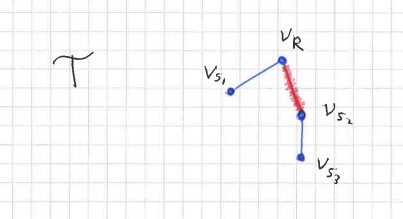
\includegraphics[angle=0,scale=0.6]{tree}
\end{figure}

Taking the double cover ramified over the blue part gives the graph $\mathcal{G}_C$ as shown:
\begin{figure} [!htb] 
%\caption{Special fibre and dual graph}
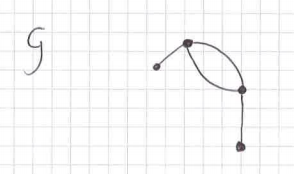
\includegraphics[angle=0,scale=0.6]{hypgraph}
\end{figure}

Note that the geometric genus of the hyperelliptic curve $\Gamma_\mathfrak{s}$ of \Cref{m2d2} is the number $g(\mathfrak{s})$ defined by
\[\#\{\textup{odd children of }\mathfrak{s}\}\in \{2g(\mathfrak{s})+2,2g(\mathfrak{s})+1\}.\]
In particular the components corresponding to $\mathcal{R}$ and $\mathfrak{s}_2$ are necessarily isomorphic to $\mathbb{P}^1$. One easily computes from  \Cref{m2d2} (iii) that the two remaining components are both given by the equation $y^2=x^3-x$ and have genus $1$. The final picture is as follows: 
\begin{figure} [!htb] 
%\caption{Special fibre and dual graph}
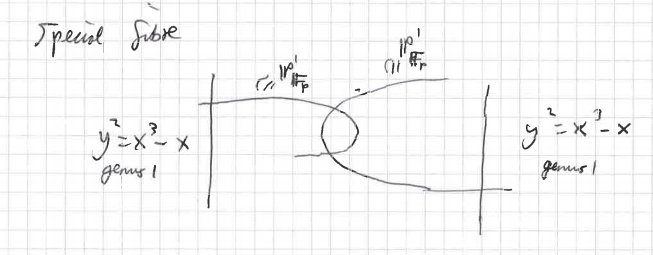
\includegraphics[angle=0,scale=0.6]{special_fibre_ex}
\end{figure}
\end{example}

%\subsection{The minimal regular model} \marginpar{at some point need to pass to max unram extension}



\subsection{The minimal regular model of a semistable hyperelliptic curve}

In the contex of \Cref{m2d2} we can additionally describe the thickness of each node in terms of the clusters and hence describe the minimal regular model of a semistable hyperelliptic curve $C/K$.

\begin{lemma}
Let $\mathcal{G}_C$ be as in  \Cref{m2d2} and let $e$ be an edge of $\mathcal{G}_C$ corresponding to clusters $\mathfrak{s}<P(\mathfrak{s})$, where $\mathfrak{s}$ has size at least $2$. Writing $\delta_\mathfrak{s}=d_{P(\mathfrak{s})}-d_\mathfrak{s}$  the thickness of the corresponding node is 
\[n(e):=\begin{cases} \delta_{\mathfrak{s}}/2~~&~~e~~\textup{came from a blue edge},\\
 \delta_\mathfrak{s}~~&~~e~~\textup{came from a yellow edge},\\
 2\delta_\mathfrak{s}~~&~~\mathfrak{s}~~\textup{a twin.}
\end{cases}\]
In particular, the dual graph of the minimal regular model of $C$ is obtained from $\mathcal{G}_C$ by replacing each edge $e$ by a path of length $n(e)$.
\end{lemma}

\begin{remark}
The condition for semistability in \Cref{m2d2} (i)  forces $\delta_\mathfrak{s}/2\in \mathbb{Z}$ in the first of the three cases above.
\end{remark}

\begin{example}
Returning to \Cref{cluster example} we find that each node has thickness $1$, so that the stable model and minimal regular model coincide.
\end{example}

\subsection{The N\'{e}ron model of an abelian variety} 

We now change tack completely and move on from models of curves to models of abelian varieties. It turns out that for an abelian variety there is always a canonical `best model', the N\'{e}ron model. As usual, let $K$ be a finite extension of $\mathbb{Q}_p$ (for $p$ arbitrary now). The standard reference for N\'{e}ron models is the book \cite{MR1045822}.


\begin{theorem} 
Let $A/K$ be an abelian variety. Then there exists a smooth\footnote{We take as our definition that a morphism $f:Y\rightarrow Z$ is \textit{smooth} if it is flat and if each fibre $Y\times_Z k(z)$ ($z\in Z$) is geometrically regular.}, separated, finite type group scheme $\mathcal{A}/\mathcal{O}_K$ with generic fibre $A$, satisfying the universal property (the \emph{N\'{e}ron mapping property}):

for each smooth $\mathcal{O}_K$-scheme $\mathcal{Y}$, any $K$-morphism $\mathcal{Y}_K\rightarrow A$ extends uniquely to an $\mathcal{O}_K$-morphism $\mathcal{Y}\rightarrow \mathcal{A}$. We call $\mathcal{A}$ the \emph{N\'{e}ron model} of $A$.
\end{theorem} 

\begin{example}
Let $E/K$ be an elliptic curve with good reduction. Then the minimal Weierstrass equation for $E$ gives the N\'{e}ron model of $E$.  
\end{example}

\begin{remark}
Note that, unlike for curves, we have dropped properness in favour of smoothness, although the N\'{e}ron mapping property forces a weak version of the valuative criterion for properness. In fact, the N\'{e}ron model is proper if and only if its special fibre is an abelian variety over $k$.
\end{remark}

\begin{defi}
The \textit{reduction} of an abelian variety over $K$ is the group variety $\mathcal{A}_k=\mathcal{A}\times_{\mathcal{O}_K}k$ over $k$. If this is an abelian variety then we say that $A/K$ has $\textit{good reduction}$. The \textit{identity component} of the N\'{e}ron model, denoted $\mathcal{A}^0$, is the open subscheme whose special fibre is the connected component of the identity $(\mathcal{A}_k)^0$ of $\mathcal{A}_k$ (i.e. remove the closed subset consisting of the union of the (finitely many) components of the special fibre not containing the identity element).   
\end{defi}

\begin{remark}
Note that the N\'{e}ron mapping property gives $A(K)=\mathcal{A}(\mathcal{O}_K)$ giving us a reduction homomorphism $A(K)\rightarrow \mathcal{A}_k(k)$. We write $A_0(K)$ for the points reducing to $\mathcal{A}_k^0(k)$. The group $A(K)/A_0(K)$ is finite and we define the \textit{Tamagawa number} $c(A/K)$ to be its order. Alternatively, if one defines $\Phi:=\mathcal{A}_k/\mathcal{A}_k^0$ (a finite etale group scheme over $k$) then one has
\[c(A/K)=\Phi(\bar{k})^{\textup{Gal}(\bar{k}/k)}.\] 
\end{remark}

\subsection{Neron models of Jacobians}

Often, one can use the existence of the N\'{e}ron model as a black box, and prove everything via the universal property. However, from a computational viewpoint this is not that satisfactory. For Jacobians however the situation is quite good since it turns out that the models of curves we have been working with are quite closely related to the N\'{e}ron  model of the Jacobian of their generic fibre. A precise result is as follows.

\begin{theorem} \label{raynauds theorem}
Let $C/K$ be a nice curve. Suppose that either
\begin{itemize}
\item $\mathcal{C}/\mathcal{O}_K$ is a semistable model of $C$,
\end{itemize}
or
\begin{itemize}
\item $\mathcal{C}/\mathcal{O}_K$ is a regular model for $C$ and the greatest common divisor of the multiplicities of the irreducible components of the special fibre of $\mathcal{C}$ is $1$.
\end{itemize}

Then $\textup{Pic}^0_{\mathcal{C}/\mathcal{O}_K}$ is canonically isomorphic to the identity component of the Neron model of the Jacobian of $C$. (The map is by extending the one on the generic fibre). 
\end{theorem}

\begin{proof}
The first part is \cite[Theorem 9.5.4 (b)]{MR1045822} whilst op. cit. Corollary 9.7.2 is the second part.
\end{proof}

\begin{cor}
Let $C/K$ be a nice curve and let $\mathcal{C}/\mathcal{O}_K$ be a model satisfying one of the two cases in \Cref{raynauds theorem}. Then the special fibre of  the identity component of the N\'{e}ron model of the Jacobian of $C$ is $\textup{Pic}^0_{\mathcal{C}_k/k}$. In particular, if $C$ has good reduction and $\mathcal{C}$ is a model for $C$ with nice special fibre, then the special fibre of the N\'{e}ron model of the Jacobian of $C$ is the Jacobian of the  special fibre of $\mathcal{C}$. 
\end{cor}

\begin{remark}
The component group, and hence Tamagawa number, can be understood via \cite[Theorem 9.6.1]{MR1045822} but this needs a regular model. 
\end{remark}

\subsection{N\'{e}ron  models of elliptic curves}

We close this section by discussing the situation for elliptic curves. Either by showing that it satisfies the N\'{e}ron mapping property, or from Raynaud's theorem, it follows that the N\'{e}ron model of an elliptic curve is the smooth part of its minimal regular model. In particular it follows e.g. from Tate's algorithm that the identity component of the Neron model is the smooth part of the minimal Weierstrass model. We have the following picture for an elliptic curve with type $I_n$ reduction:

\newpage 

\begin{figure} [!htb] 
%\caption{Special fibre and dual graph}
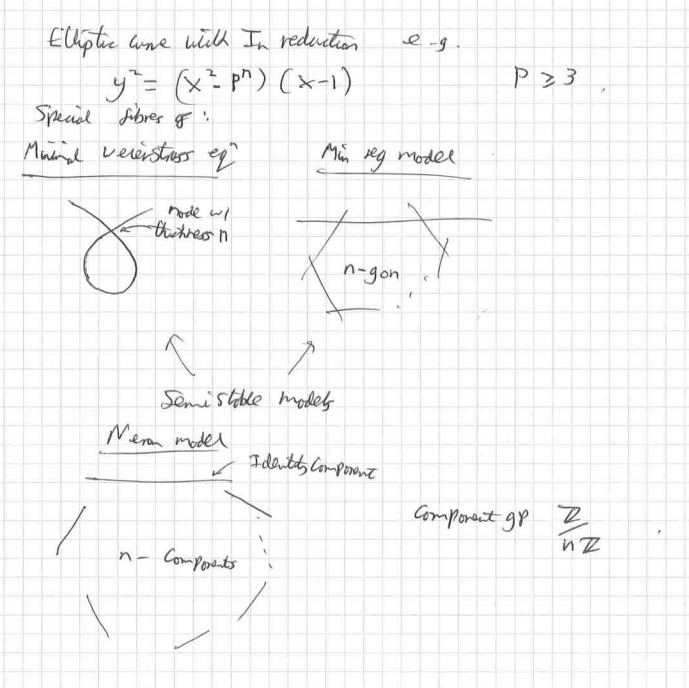
\includegraphics[angle=0,scale=0.6]{elliptic_neron}
\end{figure}


%Because of this we will often choose to pass all the way to the maximal unramified extension $K^\textup{nr}$ of $K$, so that the the residue field is algebraically closed (one could also pass to the completion of $K^\textup{nr}$ too). 
%
%On the other hand, both the N\'{e}ron model and the minimal regular model can change quite dramatically under ramified field extension (cf. elliptic curves with potentially good reduction). One of the main advantages of the stable model that it is unchanged under \textit{all} extensions. 

%
%\subsection{Unramified extensions}
%
%Both minimal regular models and N\'{e}ron models commute with unramified base change. That is, if $\mathcal{C}/\mathcal{O}_K$ is the minimal regular model of some nice curve $C$, and $F/K$ is a finite unramified extension, then $\mathcal{C}\times_{\mathcal{O}_K}\mathcal{O}_F$ is again the minimal regular model of $C$ over $F$. The analagous statement holds for the  N\'{e}ron model of an abelian variety. Roughly speaking this is due to the fact that for unramified extensions $\textup{Spec}\mathcal{O}_F\rightarrow \textup{Spec}\mathcal{O}_K$ is \'{e}tale. However, like minimal regular models, N\'{e}ron model can often change quite drastically under ramified base extension.

\newpage

\section{Exercises for Lecture 3}

\subsection{}
Let $p>3$ be a  prime and $C/\mathbb{Q}_p$ the hyperelliptic curve 
\[C:y^2=x(x-p)(x-2p)(x-3p)(x-1)(x-1+p)(x-2).\]
Show that $C/\mathbb{Q}_p$ has semistable reduction, compute the dual graph of its special fibre, and the normalisations of each of the components.


\subsection{} Find a curve $C/\mathbb{Q}_5$ which has semistable reduction, and such that the special fibre of its stable model consists of two elliptic curves meeting at a single point.

\subsection{}
Let $K$ be a finite extension of $\mathbb{Q}_p$, ring of integers $\mathcal{O}_K$, residue field $k$. Let $C/K$ be a semistable curve, $\mathcal{C}/\mathcal{O}_K$ its minimal regular model, and $\mathcal{G}$ the dual graph of (the base change to $\bar{k}$ of the special fibre of) $\mathcal{C}$. Let $L/K$ be a field extension of ramification degree $e$, and let $\mathcal{C}'$ and $\mathcal{G}'$ denote the corresponding objects over $L$. Show that $\mathcal{G}'$ is obtained from $\mathcal{G}$ by replacing each edge with a path of length $e$. 

\newpage

\newpage

\section{Lecture 4: Describing the Tate module of Jacobians}

Let $K$ be a finite extension of $\mathbb{Q}_p$ and $C/K$ a nice curve. Our aim is to understand the $l$-adic Tate module of $\textup{Jac}(C)$ for $l\neq p$.  We  consider the case where $C/K$ is semistable, although the general case can be deduced from this by keeping careful track of the action of the Galois group of some (Galois) extension over which $C$ attains semistable reduction. Note that by the semistable reduction theorem, for general $C$ this still describes the restriction of the Tate module to a finite index subgroup of $G_K$. 

\subsection{Semistable abelian varieties}

As well as a notion of semistability for curves there is a corresponding notion of semistability for abelian varieties.

\begin{defi}[Semistable abelian varieties]
Let $A/K$ be an abelian variety and $\mathcal{A}/\mathcal{O}_K$ its N\'{e}ron model. We say that $A$ has \textit{semistable reduction} over $K$ if the special fibre $A_{\bar{k}}$ of $\mathcal{A}$ is an extension of an abelian variety by a torus. In the special case where $A_{\bar{k}}$ is an abelian variety we say that $A$ has $\textit{good reduction}$.
\end{defi}

\begin{example}
An elliptic curve is semistable precisely when it has good or multiplicative reduction.
\end{example}

\begin{remark}
For the Jacobian $\textup{Jac}(C)$ of a nice curve of genus at least $2$, one can show that $\textup{Jac}(C)$ is semistable if and only if $C$ is. We'll (almost) see how to prove the implication `$C$ semistable $\Rightarrow \textup{Jac}(C)$ semistable' later in this lecture (see \Cref{semistable implies semistable jac}).
\end{remark}

\begin{remark}
As for elliptic curves, the N\'{e}ron--Ogg--Shafarevich criterion states that $A$ has good reduction if and only if $T_l(A)$ is unramified for some $l$ different from the residue characteristic of $K$. Similarly, one can show that $A$ has semistable reduction if and only if the inertia group $I_K$ acts unipotently on $T_l(A)$. 
\end{remark}

\begin{remark}
Even when $A/K$ is semistable the N\'{e}ron model still does not commte with ramified base change (consider an elliptic curve with multiplicative reduction - the order of its component group gets multiplied by the ramification degree) but it is true at least that when $A/K$ is semistable then the identity component of the  N\'{e}ron model commutes with base change. For Jacobians of curves this follows from the corresponding fact for the stable model, along with   \Cref{raynauds theorem}.
\end{remark}

\subsection{The Tate module of an abelian variety}

\subsubsection{Abelian varieties with good reduction}

Let $A/K$ be an abelian variety with good reduction and let $\mathcal{A}/\mathcal{O}_K$ be its N\'{e}ron model. Then its special fibre $\bar{\mathcal{A}}$ is an abelian variety over $k$ of dimension $g$ also. For any $l\neq \textup{char}(k)$ we have
\[\bar{\mathcal{A}}[l^n]\cong (\mathbb{Z}/l^n\mathbb{Z})^{2g}.\]
On the other hand (since N\'{e}ron models commute with unramified base change) we have a reduction map
\[A(K^\textup{nr})[l^n]\rightarrow \bar{\mathcal{A}}[l^n]\]
which is surjective by Hensel's lemma. Simply by counting we deduce that $A[l^n]\subseteq A(K^\textup{nr})$ (i.e. all $l$-power torsion in unramified) and that reduction gives an isomorphism $A[l^n]\cong \bar{\mathcal{A}}[l^n]$. In particular, $T_l(A)$ is unramified and we have a canonical isomorphism
\begin{equation} \label{tate module red 1}
 T_l(A)\cong T_l(\bar{\mathcal{A}})
\end{equation}
which is equivariant for the action of $\textup{Gal}(K^\textup{nr}/K)\cong \textup{Gal}(\bar{k}/k)$. 

In particular, if $A=\textup{Jac}(C)$ is the Jacobian of a nice curve $C$, and $C$ has good reduction (in general this is strictly stronger than $\textup{Jac}(C)$ having good reduction) then we have a canonical isomorphism
\begin{equation} \label{jac tate module}
 T_l(\textup{Jac}(C))\cong T_l(\textup{Jac}(\bar{\mathcal{C}})) 
\end{equation}
equivariant for the action of $\textup{Gal}(K^\textup{nr}/K)\cong \textup{Gal}(\bar{k}/k)$, where here $\mathcal{C}$ is the model of $C$ realising the good reduction. This means that the local $L$-polynomial of $\textup{Jac}(C)$ is completely determined by the action of Frobenius on $H^1_{\textup{et}}(\bar{\mathcal{C}}_{\bar{k}},\mathbb{Z}_l)$, and this may be understood by the Weil conjectures in terms of the number of points on $\bar{\mathcal{C}}$ over finite extensions of $k$. See Andrew Sutherland's course for more on this.

\begin{remark}
An alternative viewpoint of \Cref{jac tate module} is that it follows as a special case of the smooth and proper base change theorems in \'{e}tale cohomology applied to the scheme $\mathcal{C}/\mathcal{O}_K$ (which is smooth and proper over $\mathcal{O}_K$ under our good reduction assumption).
\end{remark}

\subsubsection{Semistable abelian varieties}

We now move on to the case where $A/K$ has semistable but not necessarily good reduction. It turns out, though it is harder to prove, that the analogue of \Cref{tate module red 1} is that there is a $\textup{Gal}(K^\textup{nr}/K)=\textup{Gal}(\bar{k}/k)$ equivariant isomorphism
\begin{equation}\label{tate module red 2}
T_l(A)^{I_K}\cong T_l(\bar{\mathcal{A}}^0)
\end{equation}
where here $I_K$ denotes the inertia group of $K$. In fact, this holds in general without the assumption that $A/K$ is semistable though we will not persue that further.

\subsection{The Picard group of semistable curves}

In light of \Cref{tate module red 2}, we want to describe  $T_l(\bar{\mathcal{A}}^0)$ in the case that $A=\textup{Jac}(C)$ is the Jacobian of a nice curve $C/K$. Supposing that $C/K$ is semistable, by \Cref{raynauds theorem} we have $T_l(\bar{\mathcal{A}}^0)=T_l(\textup{Pic}^0(\bar{\mathcal{C}}))$ where $\mathcal{C}/\mathcal{O}_K$ is the stable model of $C$. It is this group which we now describe. We begin by describing the Picard group of an arbitrary  semistable curve $X$ over an algebraically closed field.

It will be convenient to begin with a slight refinement of the definition of the dual graph.

\begin{defi}[Dual graph, take two]
As usual, let $\pi:\tilde{X}\rightarrow X$ be the normalisation morphism and write 

\begin{tabular}{llllll}
$S$        &=& set of singular (ordinary double) points of $X$,\cr
$T$        &=& set of connected components of $\tilde{X}$,\cr
$R$        &=& $\pi^{-1}(\mathcal{S})$; this comes with two canonical maps\cr
&& $\phi:R\to S$, $P\mapsto\pi(x),$\cr
&& $\psi: R\to R$, $P\mapsto$ component of $\tilde{X}$ on which $x$ lies.\cr
\end{tabular}

\noindent The dual graph $\mathcal{G}$ of $X$ has vertex set $T$ and edge set $S$. $R$ is thought of as the set of edge endpoints, and the maps $\phi$ and $\psi$ specify adjacency.  Note that a graph automorphism of $\mathcal{G}$ (which we allow to permute multiple edges and swap edge endpoints) is precisely
the data of bijections $R\to R$, $S\to S$ and $T\to T$ that commute with $\phi$ and $\psi$.
\end{defi}

The following proposition reduces understanding the Tate module $T_l  \textup{Pic}^0(X)$ assocaited to a semistable curve, to understanding the Tate module of the Jacobians of the normalisations of its irreducible components, along with the (co)homology group of its dual graph. 

\begin{proposition}
Let $X$ be a semistable curve over $k=\bar{k}$ and $\mathcal{G}$ its dual graph. Then for each prime $l\neq\textup{char}(k)$ we have an exact sequence
$$
  0 \longrightarrow H^1(\mathcal{G},\mathbb{Z}) \otimes_\mathbb{Z}\mathbb{Z}_l(1) \longrightarrow T_l  \textup{Pic}^0(X) \longrightarrow\prod_{\Gamma \in \mathcal{J}} T_l (\textup{Jac}(\Gamma)) \longrightarrow 0
$$
where $H^1(\mathcal{G},\mathbb{Z})$ denotes the first singular cohomology group\footnote{We view the graph $\mathcal{G}$ as a topological space in the obvious way, by thinking of each edge as an interval on the real line.} of the graph $\mathcal{G}$.
\end{proposition}

\begin{proof}[Proof (sketch)]
 We consider \Cref{first sheaf seq} where we replace the structure sheaf with the invertible elements of the structure sheaf. Thus we obtain
\begin{equation*}\label{second sheaf seq} 
0\longrightarrow \mathcal{O}_X^\times\longrightarrow \pi_*(\mathcal{O}_{\tilde{X}}^\times)\longrightarrow \mathcal{F}\longrightarrow 0
\end{equation*}
where again $\mathcal{F}$ is defined by the sequence and is a skyscraper sheaf supported on $X_\textup{sing}$. The associated sequence for cohomology gives 
\begin{equation*}\label{second sheaf seq} 
0\longrightarrow \mathcal{O}_X^\times (X)\longrightarrow \mathcal{O}_{\tilde{X}}^\times(X)\longrightarrow \mathcal{F}(X)\longrightarrow \textup{Pic}(X)\longrightarrow \prod_{\Gamma \in T}\textup{Pic}(\Gamma) \longrightarrow 0.
\end{equation*}
Now $\mathcal{O}_X^{\times}(X)=k^\times$ since $X$ is proper and connected, whilst $\mathcal{O}_{\tilde{X}}^\times(X)=(k^\times)^S$ (functions from $S$ to $k^\times$), and the map $\mathcal{O}_X^{\times}(X) \longrightarrow \mathcal{O}_{\tilde{X}}^\times(X)$ sends an element of $k^\times$ to the constant function with this value. On the other hand, $\mathcal{F}(X)=\oplus_{x\in S}\mathcal{F}_x$ and using the fact that each element of $S$ is an ordinary double point we find that 
\[\mathcal{F}(X)=\textup{coker}\left((k^\times)^S\stackrel{\phi^*}{\longrightarrow}(k^\times)^R\right)\]
where $\phi^*$ is pullback of functions.  Bringing the above discussion together, and restricting to degree $0$ line bundles, we have an exact sequence
\begin{equation}\label{good pic sequence}
0\longrightarrow k^\times \stackrel{\Delta}{\longrightarrow} (k^\times)^T\stackrel{\psi^*}{\longrightarrow}\frac{(k^\times)^R}{\phi^*\left((k^\times)^S\right)}\longrightarrow \textup{Pic}^0(X)\longrightarrow \prod_{\Gamma \in T}\textup{Jac}(\Gamma)(k)\longrightarrow 0
\end{equation}
where $\Delta$ is the diagonal embedding.

On the other hand, if we write $\mathcal{G}=U\cup V$ where $U$ is the union of open edges and $V$ is the union of small open neighbourhoods of the vertices then Mayer--Vietoris gives 
\begin{equation}
0\longrightarrow H_1(\mathcal{G},\mathbb{Z})\longrightarrow \mathbb{Z}^R\stackrel{(\phi,\psi)}{\longrightarrow}\mathbb{Z}^{S}\oplus \mathbb{Z}^{T}\longrightarrow \mathbb{Z}\longrightarrow 0
\end{equation}
since $H_0(U)=\mathbb{Z}^S$, $H_0(V)=\mathbb{Z}^T$, $H_0(U\cap V)=\mathbb{Z}^R$ and all higher homology groups vanish. Applying $\textup{Hom}\left(-,\mathbb{Z}_l(1)\right)$ to this sequence, and comparing the result with the sequence of Tate modules obtained from \Cref{good pic sequence}, gives the result.
\end{proof}

\begin{remark}
If each component of $X$ has arithmetic genus $0$, as is the case for the curves of \Cref{dual graph ex 1,dual graph ex 2}, then the proposition gives a canonical isomorphism 
\[H^1(\mathcal{G},\mathbb{Z}) \otimes_\mathbb{Z}\mathbb{Z}_l(1)\cong  T_l  \textup{Pic}^0(X).\]
\end{remark}

\begin{remark} \label{semistable implies semistable jac}
The exact sequence \Cref{good pic sequence} describes $\textup{Pic}^0(X)$ on the level of $k$-points. However, one can ramp this argument up to give a description of the identity component of the relative Picard functor $\textup{Pic}^0_{X/k}$ as an algebraic group. In fact, this shows that $\textup{Pic}^0_{X/k}$ is an extension of an abelian variety, namely $\prod_{\Gamma \in \mathcal{I}}\textup{Jac}(\Gamma)$, by a torus of dimension equal to the rank of $H_1(\mathcal{G},\mathbb{Z})$. In particular, this shows that the Jacobian of a semistable curve over a local field has semistable reduction.
\end{remark}

\subsection{Computation of local factors of $L$-functions}

Now return to the case where $K$ is a finite extension of $\mathbb{Q}_p$, $l$ a prime $\neq p$, and $C/K$ a nice curve with semistable reduction, and denote by $J$ its Jacobian. Fixing a semistable model $\mathcal{C}/\mathcal{O}_K$ for $C$, and let $\mathcal{G}$ be the dual graph of $\mathcal{C}_{\bar{k}}$. We get as a corollary of the above discussion (the $G_k$-action on $\mathcal{G}$ coming from the actions on the sets $S$, $T$ and $R$ above, and $\Gamma$ denotes an irreducible component of $\mathcal{C}_{\bar{k}}$ and $\widetilde{\Gamma}$ its normalisation):

\begin{cor}
Denoting $\tilde{C}_{\bar{k}}$ the normalisation of $\mathcal{C}_{\bar{k}}$, we have a short exact sequence of $G_k$-modules
$$
  0 \longrightarrow H^1(\mathcal{G},\mathbb{Z}) \otimes_\mathbb{Z}\mathbb{Z}_l(1) \longrightarrow T_l(J)^{I_K} \longrightarrow \bigoplus_{G_k-\textup{orbs of cmps }\Gamma}\textup{Ind}_{\textup{Stab}(\Gamma)}^{G_k} T_l (\textup{Jac}(\widetilde{\Gamma})) \longrightarrow 0.
$$
\end{cor}

Recall that the local $L$-polynomial of $J/K$ defined as
\[L(J/K,T)=\textup{det}\left(1-\textup{Frob}_K^{-1}T\mid ((V_lJ)^\vee)^{I_K}\right).\]

\begin{cor}
We have
\[L(J/K,T)=\textup{det}\left(1-\textup{Frob}_{K}^{-1}T~\big\lvert ~H_1(\mathcal{G},\mathbb{Q}_l)\oplus \bigoplus_{G_k-\textup{orbs of cmps }\Gamma}\textup{Ind}_{\textup{Stab}(\Gamma)}^{G_k} T_l (\textup{Jac}(\widetilde{\Gamma})) \right).\]
\end{cor}

\begin{proof}
The Weil pairing $T_l\times T_l\rightarrow \mathbb{Z}_l(1)$ gives 
\[T_l(J)^\vee \cong T_l(J)(-1)\]
where the $(-1)$ denotes a Tate twist. Since $\mathbb{Z}_l(1)$ is unramified we can take inertia invariants to find
\[T_l(J)^\vee \cong T_l(J)^{I_K}(-1).\]
It just remains to twist the statement of the above corollary by $-1$, $\otimes_{\mathbb{Z}_l}\mathbb{Q}_l$ and note that 
\begin{itemize}
\item characteristic polynomials depend only on the semisimplification of a representation
\item $H^1(\mathcal{G},\mathbb{Q}_l)$ and $H_1(\mathcal{G},\mathbb{Q}_l)$ are isomorphic representations.
\end{itemize}
\end{proof}

\begin{example}
As a (very) special case of the above, take an elliptic curve $E$ over $K$ with multiplicative reduction. Take as our semistable model the minimal Weierstrass model, so that its special fibre is a nodal cubic curve. In particular, the Jacobian of the normalisation of the special fibre is (the Jacobian of $\mathbb{P}^1$) $0$, and $H_1(\mathcal{G},\mathbb{Q}_l)$ is isomorphic to $\mathbb{Q}_l$ with $G_k$ acting trivially if $E$ has split multiplicative reduction, and with $\textup{Frob}$ acting as multiplication by $-1$ in the case of non-split reduction. Applying the corollary we find
\[L(E,T)=\begin{cases}
1-T~~&~~E\textup{ has split multiplicative reduction}\\
1+T~~&~~E\textup{ has non-split multiplicative reduction}.
\end{cases}.\]
\end{example}

\newpage

\section{Exercises for lecture 4}

\subsection{} Let $C/\mathbb{Q}$ be the genus $3$ hyperelliptic curve 
\[C:y^2=x\left(x^2-2x-8\right)\left(x^4-16x^2+100\right).\]
Compute the local factor of the $L$-function of the Jacobian of $C$ over $\mathbb{Q}_3$. 

\textit{Hint: for a `singular hyperelliptic curve' $X:y^2=f_1(x)f_2(x)^2$ over a field $k$, where $f_1(x)$ and $f_2(x)$ are coprime square free polynomials, the normalisation $\tilde{X}$ of $X$ is the the curve
\[\tilde{X}:y^2=f_1(x)\]
and the normalisation map $\pi:\tilde{X}\rightarrow X$ is given by
\[\pi(x,y)=\left(x,yf_2(x)\right).\]}

\subsection{} For an elliptic curve $E$ having split multiplicative reduction over a local field $K$, a result of Tate gives an isomorphism
\[E(\bar{K})\cong \bar{K}^\times/q^\mathbb{Z},\]
equivariant for the natural $G_K$-actions on each side,
where $q\in K$ is an element of valuation $\geq 1$. Use this to give another proof that the local factor of the $L$-function of $E/K$ is
\[L(E/K,T)=\begin{cases}
1-T~~&~~E\textup{ has split  multiplicative reduction}\\
1+T~~&~~E\textup{ has non-split multiplicative reduction}.
\end{cases}\]

\newpage 

%\newpage
%
%\section{Exercises}
%
%\subsection{}
%Let $k$ be an algebraically closed field of characteristic different from $2$, and let $C:y^2=f(x)$ be a hyperelliptic curve over $k$ where $f(x)$ has odd degree $2g+1$ ($g\geq 2$). Denote by $\mathcal{R}$ the set of roots of $f(x)$.
%\begin{itemize}
%\item[(i)] Show that the ramification points of the $x$-coordinate map $\phi:C\rightarrow \mathbb{P}^1$ are the points $P_r=(r,0)$ for $r\in \mathcal{R}$, along with the unique point $O$ at infinity.
%\item[(ii)] Show that each of the degree $0$ divisors \[\{P_r-O~~\mid ~~r\in \mathcal{R}\}\] are $2$-torsion points in the Jacobian of $C$.
%\item[(iii)] Show that, for $k$ now not necessarily algebraically closed, as a $\textup{G}_k$-module, the $2$-torsion subgroup of the Jacobian of $C$ is isomorphic to
%\[\mathbb{F}_2[\mathcal{R}]_{\Sigma=0}\]
%where $\mathbb{F}_2[\mathcal{R}]$ denotes the permuation module on $\mathcal{R}$ with $\mathbb{F}_2$-coefficients, and $\Sigma$ is the sum-of-coordinates map.
%\item[(iv)] What is the analagous description in the case where $f(x)$ has even degree?
%\end{itemize}
%
%\subsection{}
%Let $k$ be an algebraically closed field of characteristic different from $2$, and let $C:y^2=f(x)$ be a hyperelliptic curve over $k$ of genus $2$ (so that $f$ has degree 5 or 6). Denote by $\iota$ the \textit{hyperelliptic involution} sending a point $P=(x,y)$ to $(x,-y)$. 
%\begin{itemize}
%\item[(i)] Show that the class of the canonical divisor $K_C$ is represented by the divisor $P+\iota(P)$ for any point $P$ on $C$ (hint: consider the degree $2$ map to $\mathbb{P}^1$ and use Riemann--Hurwitz).
%\item[(ii)] Show that the map sending  $\{P_1,P_2\}$  to the divisor $P_1+P_2-O-\iota(O)$ (for $O$ any point at infinity) is a surjection from the set of unordered pairs of points on $C$ to the set degree $0$ divisors on $C$ modulo linear equivalence. Show that the inverse image of any degree $0$ divisor class other than $0$ consists of a unique pair. What is the inverse image of the $0$ class? (Note that for a general (say perfect) field $k$ this gives a description of $\textup{Jac}(C)(\bar{k})$ as a $G_k$-set.)
%\item[(iii)] How would one go about adding two points $\{P_1,P_2\}$ and $\{Q_1,Q_2\}$ of $\textup{Jac}(C)$ via this identification?
%\end{itemize}
%
%\subsection{}
%Let $p$ be odd and $C/\mathbb{Q}_p:y^2=f(x)$ be a hyperelliptic curve where $f(x)$ is monic and has coefficients in $\mathbb{Z}_p$. Suppose that the discriminant of $f(x)$ has $p$-adic valuation $1$. Show that the scheme over $\mathbb{Z}_p$ given by glueing the usual charts
%\[\textup{Spec }\mathbb{Z}_p[x,y]/(y^2-f(x))\]
%and
%\[\textup{Spec }\mathbb{Z}_p[w,z]/(z^2-w^{2g+2}f(1/w))\] 
%via $x=1/w$ and $y=w^{g+1}z$ gives both a regular and semistable model of $C$ (in particular, this is the minimal regular model of $C$).
%
%\subsection{}
%Justify \Cref{plane curve example}: let $X$ be an affine plane curve given by an equation $\{f(x,y)=0\}\subseteq \mathbb{A}^2$ and suppose that $(0,0)\in X$. Write 
%\[f(x,y)=a_1x+a_2y+b_1x^2+b_2xy+b_3y^2+...\]
%Show that $(0,0)$ is a singular point of $X$ if and only if $a_1=0=a_2$. Supposing $(0,0)$ is singular, compute the completed local ring at $(0,0)$ in the case that the discriminant
%\[b_2^2-4b_1bb_3\]
%of the quadratic term is non-zero, and deduce that $(0,0)$ is an ordinary double point. 
%
%\subsection{}
%Let $p>3$ be a  prime and $C/\mathbb{Q}_p$ the hyperelliptic curve 
%\[C:y^2=x(x-p^5)(x-p)(x-3p)(x-1)(x-1+p)(x-2)(x-2+p).\]
%Show that $C/\mathbb{Q}_p$ is semistable, compute its dual graph, and the normalisations of each of the components of its special fibre.
%
%
%
%\subsection{}
%
%Let $K$ be a local field and $C/K$ be a semistable curve. Let $\mathcal{C}/\mathcal{O}_K$ be its minimal regular model and $\mathcal{G}$ the dual graph of (the special fibre of) $\mathcal{C}$. Let $L/K$ be a field extension of ramification degree $e$, and let $\mathcal{C}'$ and $\mathcal{G}'$ denote the corresponding objects over $L$. Show that $\mathcal{G}'$ is obtained from $\mathcal{G}$ by replacing each edge with a path of length $e$. 
%\newpage

\bibliographystyle{plain}

\bibliography{references}

\end{document}